\chapter[Timing Results and Analysis]{Timing Synchronization Results and Analysis}
\label{chap:timing_results}

This chapter presents the experimental evidence for the first three research questions. EXP01 verifies the baseline OFDM link, EXP02 isolates the effects of imposed timing offsets, and EXP03--06 provide individual estimator checks. The primary comparison is EXP07, which applies the common experimental conditions described in Chapter~\ref{chap:methodology}. Results in this chapter are obtained from the saved simulation outputs. The additional descriptive plots and tables are computed from those outputs without generating new transmission or noise realizations.

\section[Baseline Verification]{Baseline Verification of the OFDM Link}
\label{sec:ch4_baseline}
EXP01 first tests the QPSK--OFDM transmitter and receiver under perfect synchronization in AWGN. For each useful-data $E_b/N_0$ value, 1,000 OFDM symbols (128,000 bits) are evaluated. Figure~\ref{fig:ch4_baseline} compares the observed BER with the coherent QPSK reference in Eq.~(2.4). At 0 dB, the simulated BER is 0.077664, compared with the theoretical value 0.078650. At 4 dB the corresponding values are 0.012305 and 0.012501; at 8 dB, 20 errors yield a BER of 0.00015625, against a theoretical value of approximately $1.91\times10^{-4}$.

\begin{figure}[!htbp]
\centering
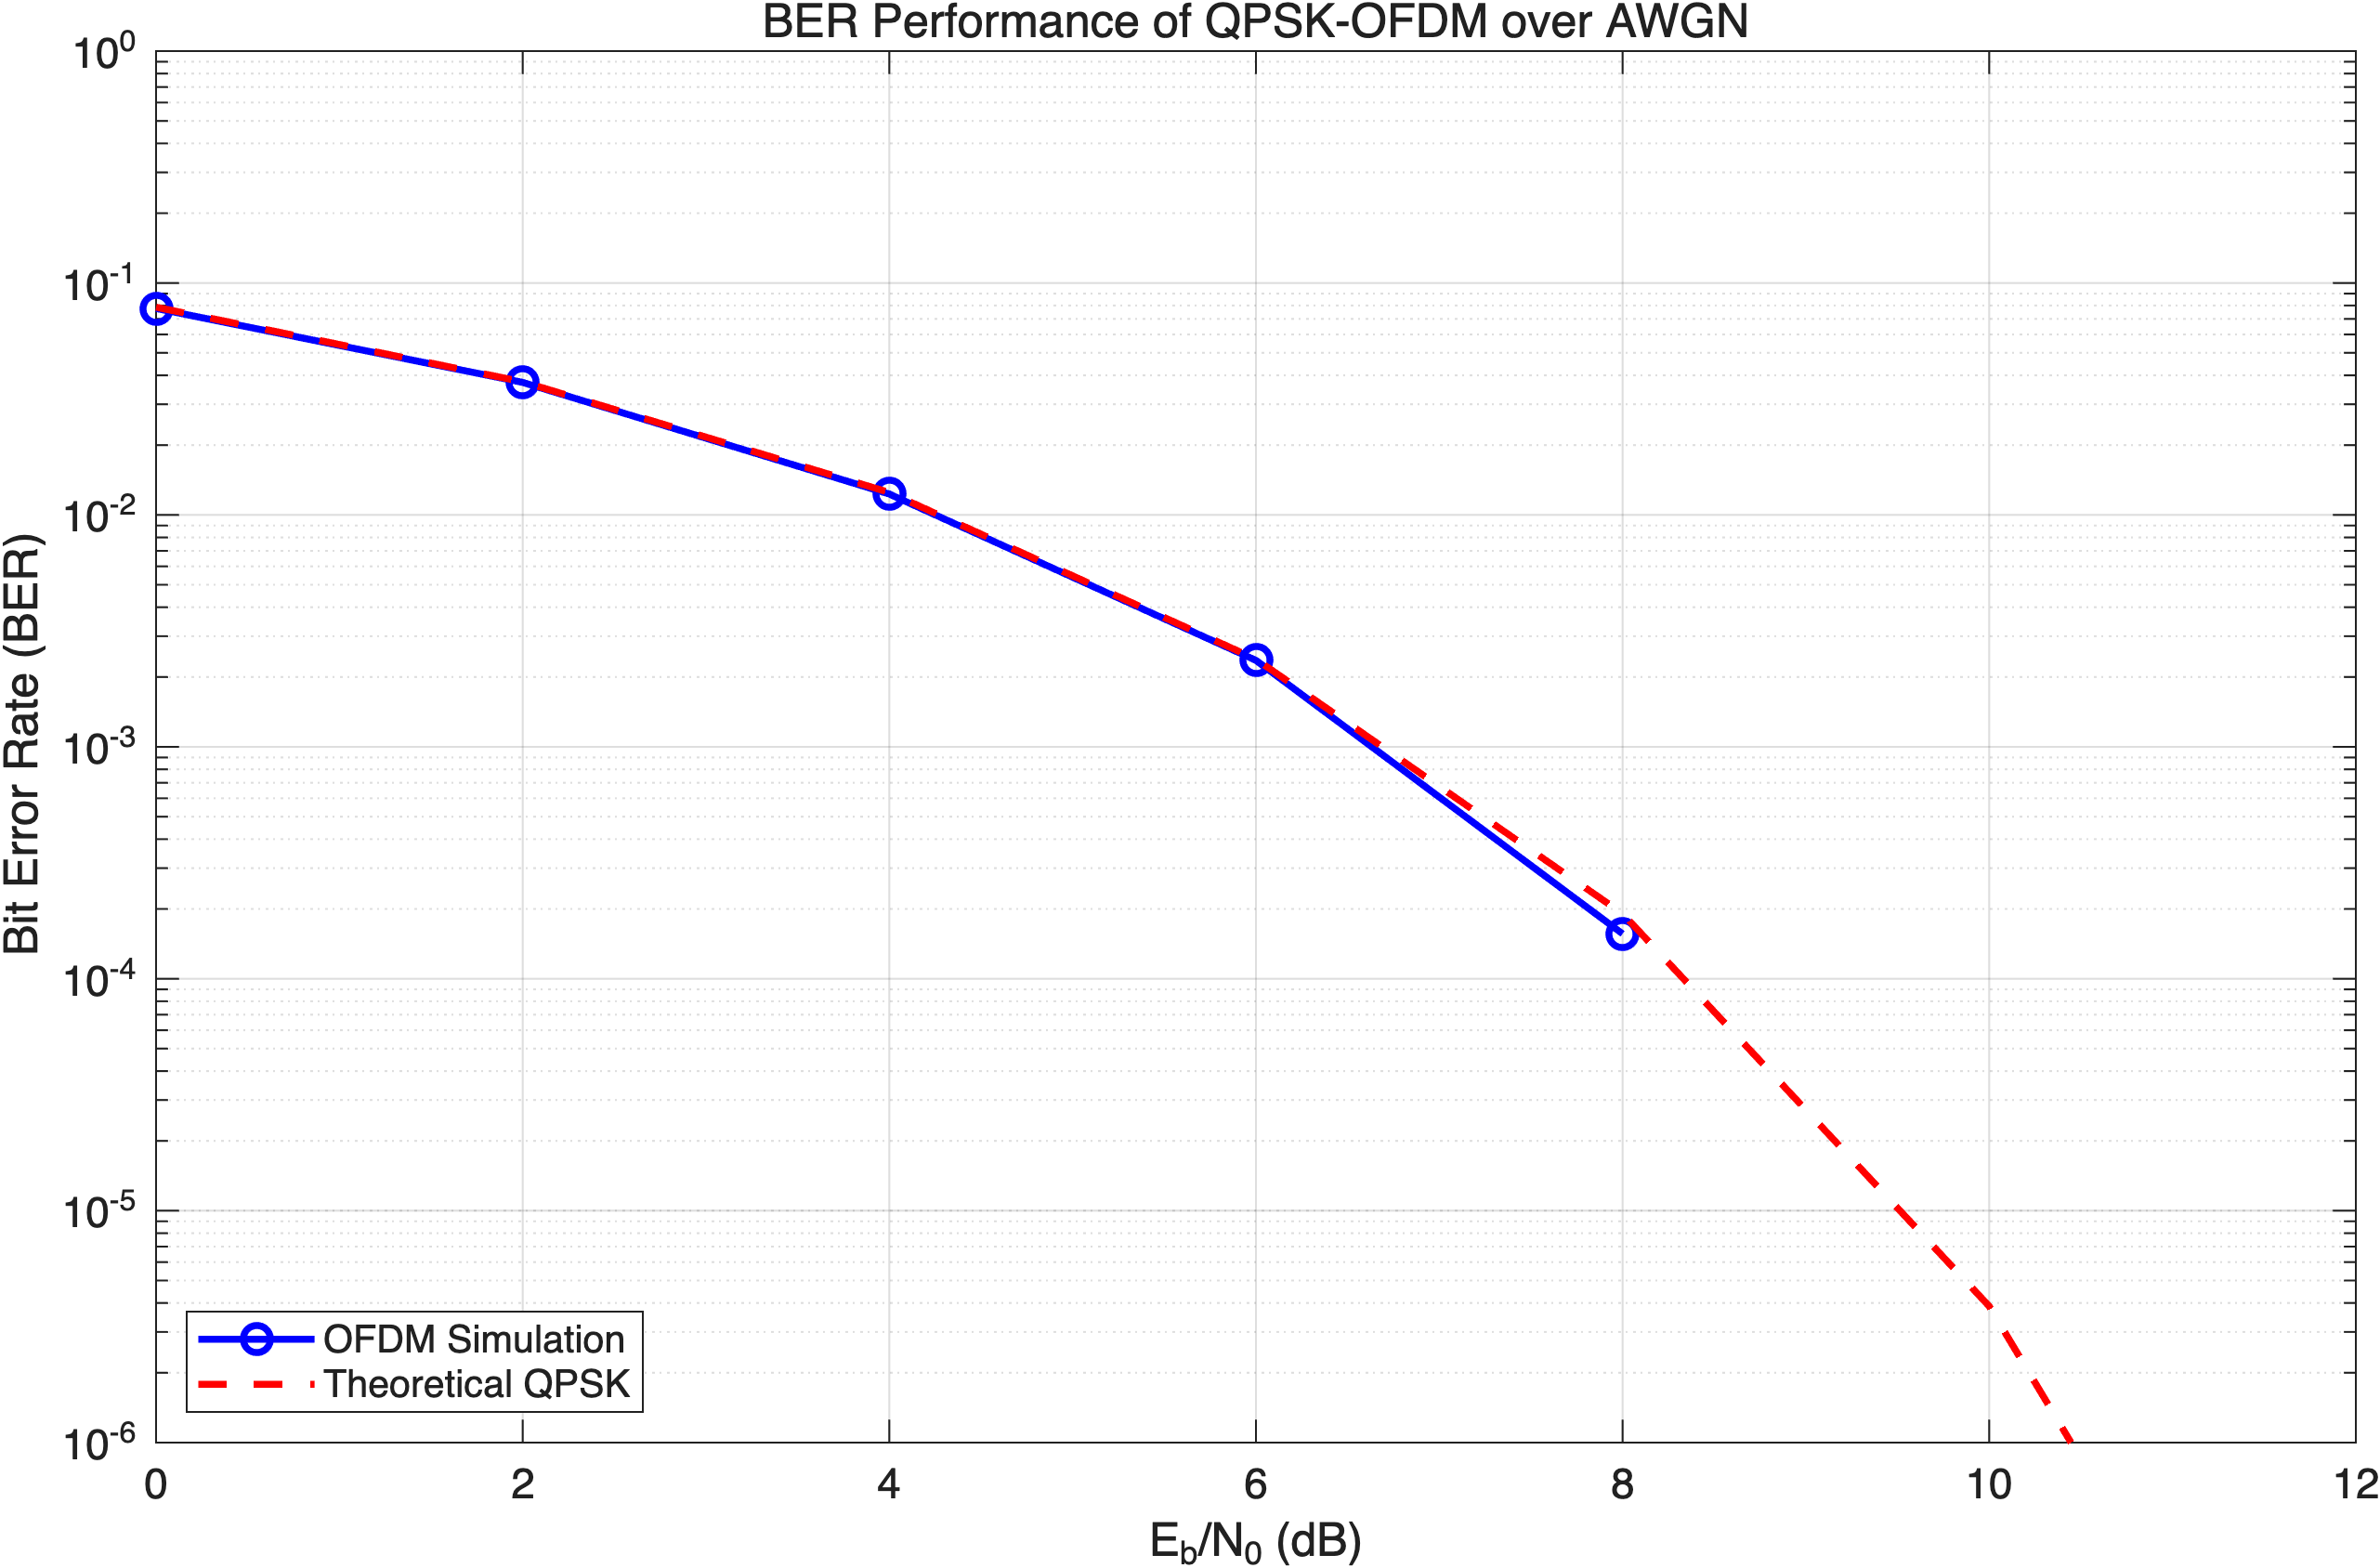
\includegraphics[width=.88\linewidth]{figures/ch4/exp01_ber_vs_ebn0.png}
\caption{EXP01: baseline QPSK--OFDM BER in AWGN. The logarithmic plot omits simulated zero-error observations and shows the low-$E_b/N_0$ range.}
\label{fig:ch4_baseline}
\end{figure}

The numerical agreement at low and moderate $E_b/N_0$ supports the consistency of modulation, IFFT/FFT processing, CP removal and the noise convention used in the baseline. No bit errors are observed from 10 through 20 dB. This does not establish zero theoretical BER: for example, the theoretical probability at 10 dB is $3.87\times10^{-6}$, corresponding to fewer than one expected error in 128,000 bits. The finite experiment therefore cannot resolve very small probabilities. The baseline horizontal axis is useful-data $E_b/N_0$, not the received active-frame SNR of EXP07.

\section[Controlled Timing Offsets]{Sensitivity to Controlled Timing Offsets}
\label{sec:ch4_offset}
EXP02 imposes known integer displacements of the FFT window rather than obtaining them from an estimator. This isolates the receiver's response to timing error. The noiseless frequency-domain experiment scans offsets from $-24$ to $+24$ samples. As shown in Figure~\ref{fig:ch4_offset_mse}, nonzero offsets within the single-path CP-safe region produce frequency-domain MSE of 2 (relative to unit-energy transmitted subcarrier symbols), despite preserving subcarrier magnitudes. Indeed, for a nonzero integer shift $e$ with $|e|<N$, the geometric-sum identity gives
\begin{equation}
\frac{1}{N}\sum_{k=0}^{N-1}\left|\exp(j2\pi ke/N)-1\right|^2=2.
\end{equation}
This is a symbol-domain error measure, not the timing-estimation MSE in samples squared. The distinction is important throughout the chapter.

\begin{figure}[!htbp]
\centering
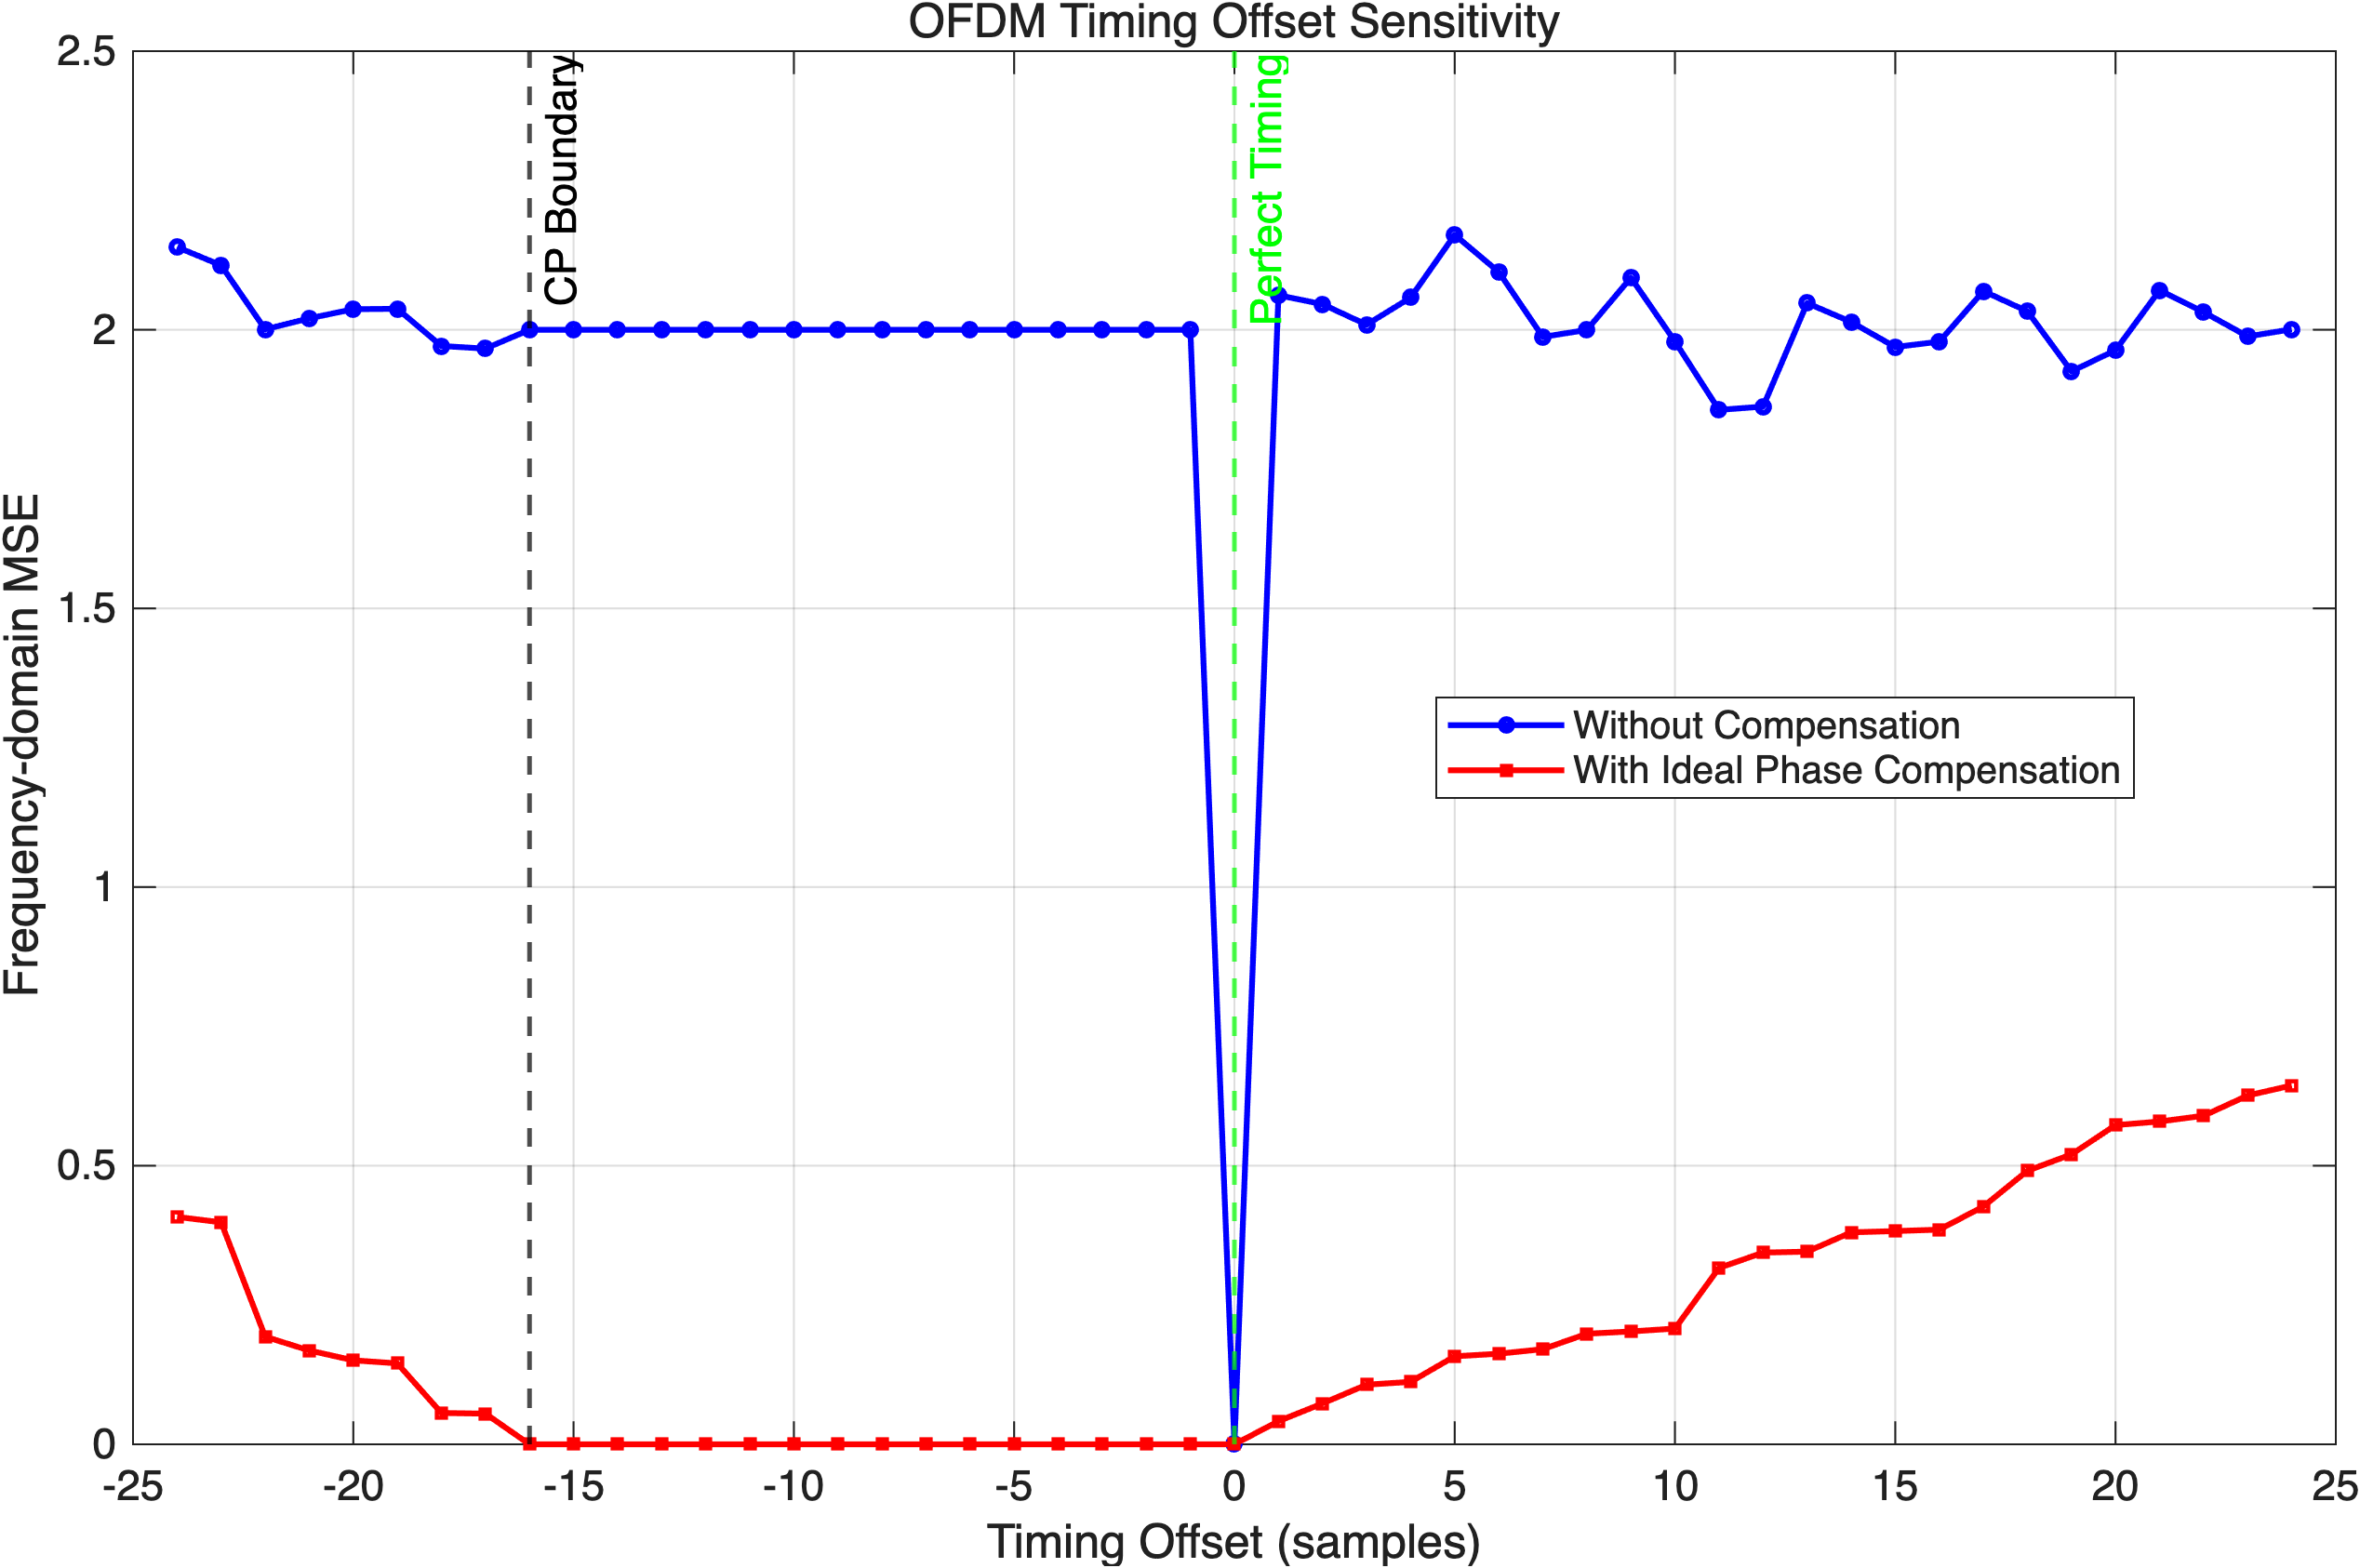
\includegraphics[width=.88\linewidth]{figures/ch4/exp02_timing_offset_sensitivity.png}
\caption{EXP02: noiseless frequency-domain MSE with and without phase compensation.}
\label{fig:ch4_offset_mse}
\end{figure}

At $e=-5$, the uncompensated frequency-domain MSE is 2, while phase compensation reduces it to approximately $1.78\times10^{-30}$. At $e=+5$, the compensated MSE remains approximately 0.1579. The latter window includes samples beyond the current useful symbol; thus the ideal circular-shift relation cannot account for the entire observation. The boundary at $-16$ is likewise visible in the compensated MSE curve.

The noiseless BER scan in Figure~\ref{fig:ch4_offset_ber} confirms the detection consequences. At $e=-5$, uncompensated BER is 0.498680, whereas compensation yields zero observed errors; at $e=+5$, the compensated BER is 0.008422. At $e=+24$ it rises to 0.215477. Some offsets outside the safe region still yield zero observed errors after compensation (for example, $e=-18$), but the frequency-domain distortion is nonzero. The CP-safe criterion is a sufficient structural condition, not a necessary condition for every finite set of QPSK decisions to be correct.

\begin{figure}[!htbp]
\centering
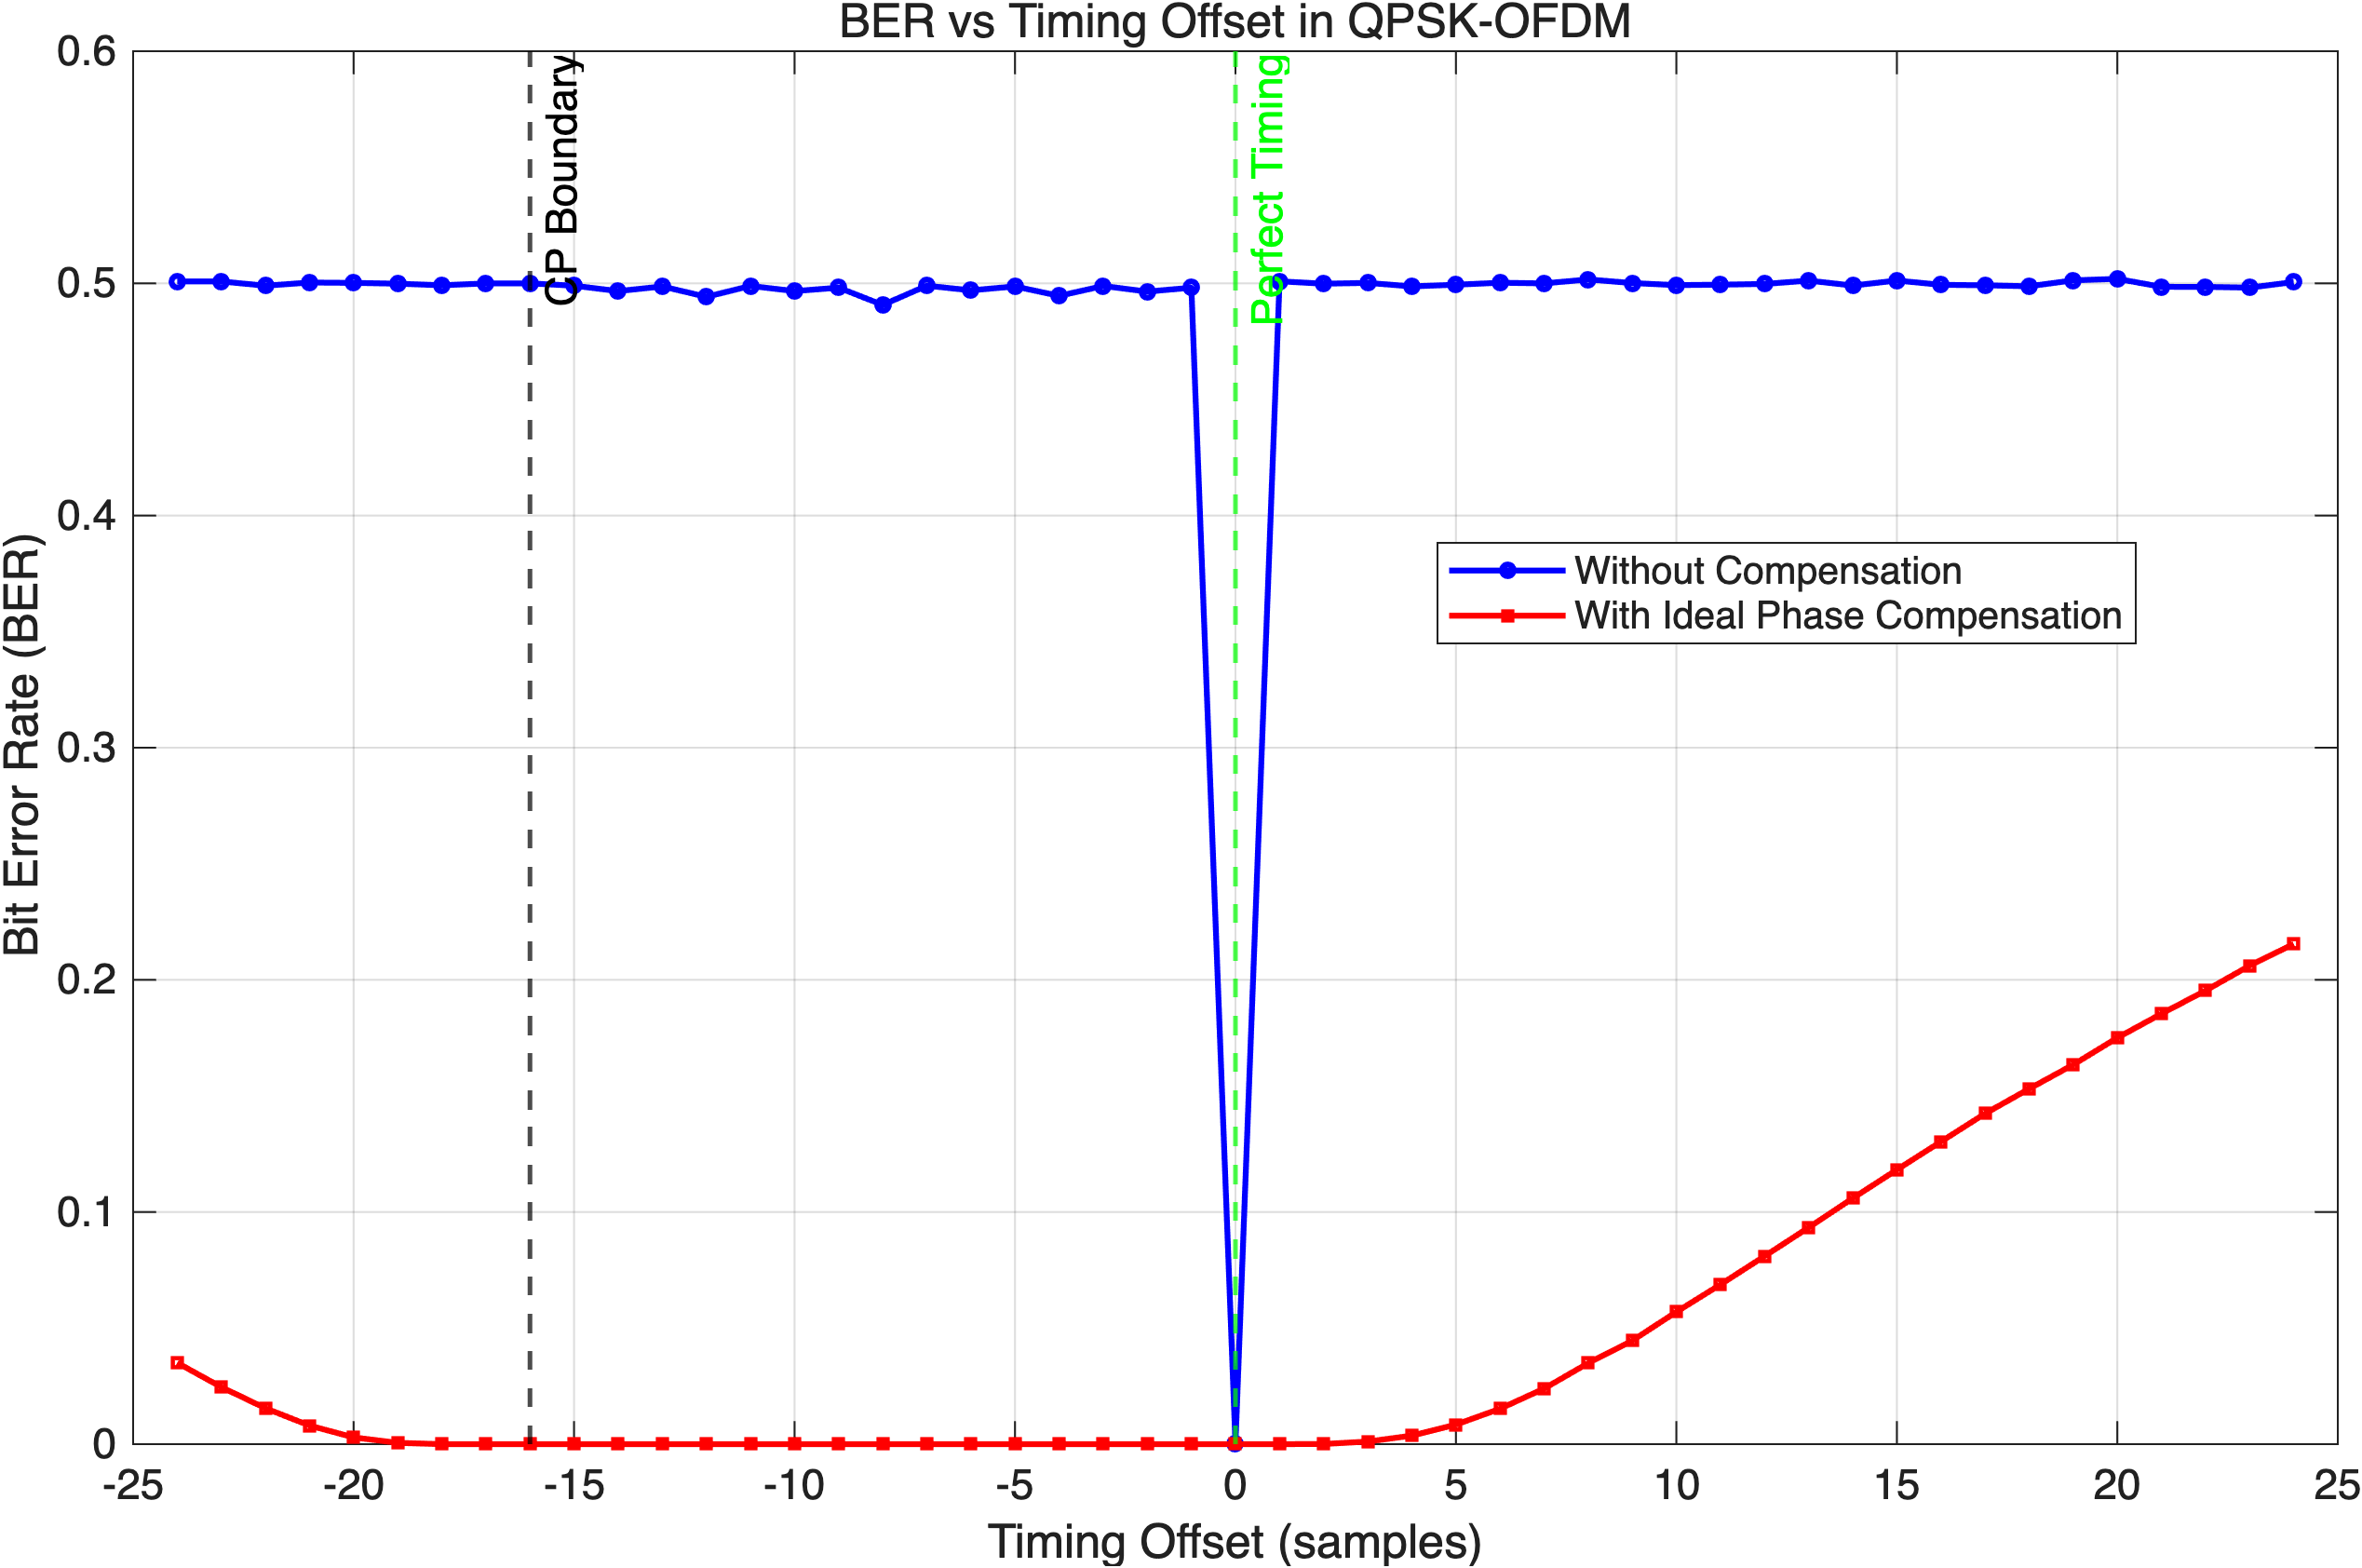
\includegraphics[width=.88\linewidth]{figures/ch4/exp02_ber_vs_timing_offset.png}
\caption{EXP02: noiseless BER for imposed FFT-window displacements, using 128,000 data bits.}
\label{fig:ch4_offset_ber}
\end{figure}

A separate AWGN experiment compares the perfect window, a five-sample early window with and without phase compensation, and a five-sample late window with compensation. Figure~\ref{fig:ch4_offset_snr} shows that the compensated early window closely tracks perfect timing. At $E_b/N_0=8$ dB, both record 21 bit errors, while the late compensated window records 3,292. At 12 dB, the perfect and compensated early cases record no errors, but the late compensated case records 1,898 (BER 0.014828). Uncompensated early-window BER stays close to 0.5. These results support the phase-rotation explanation of Chapter 2 and motivate a separate evaluation of CP-safe and exact timing probabilities.

\begin{figure}[!htbp]
\centering
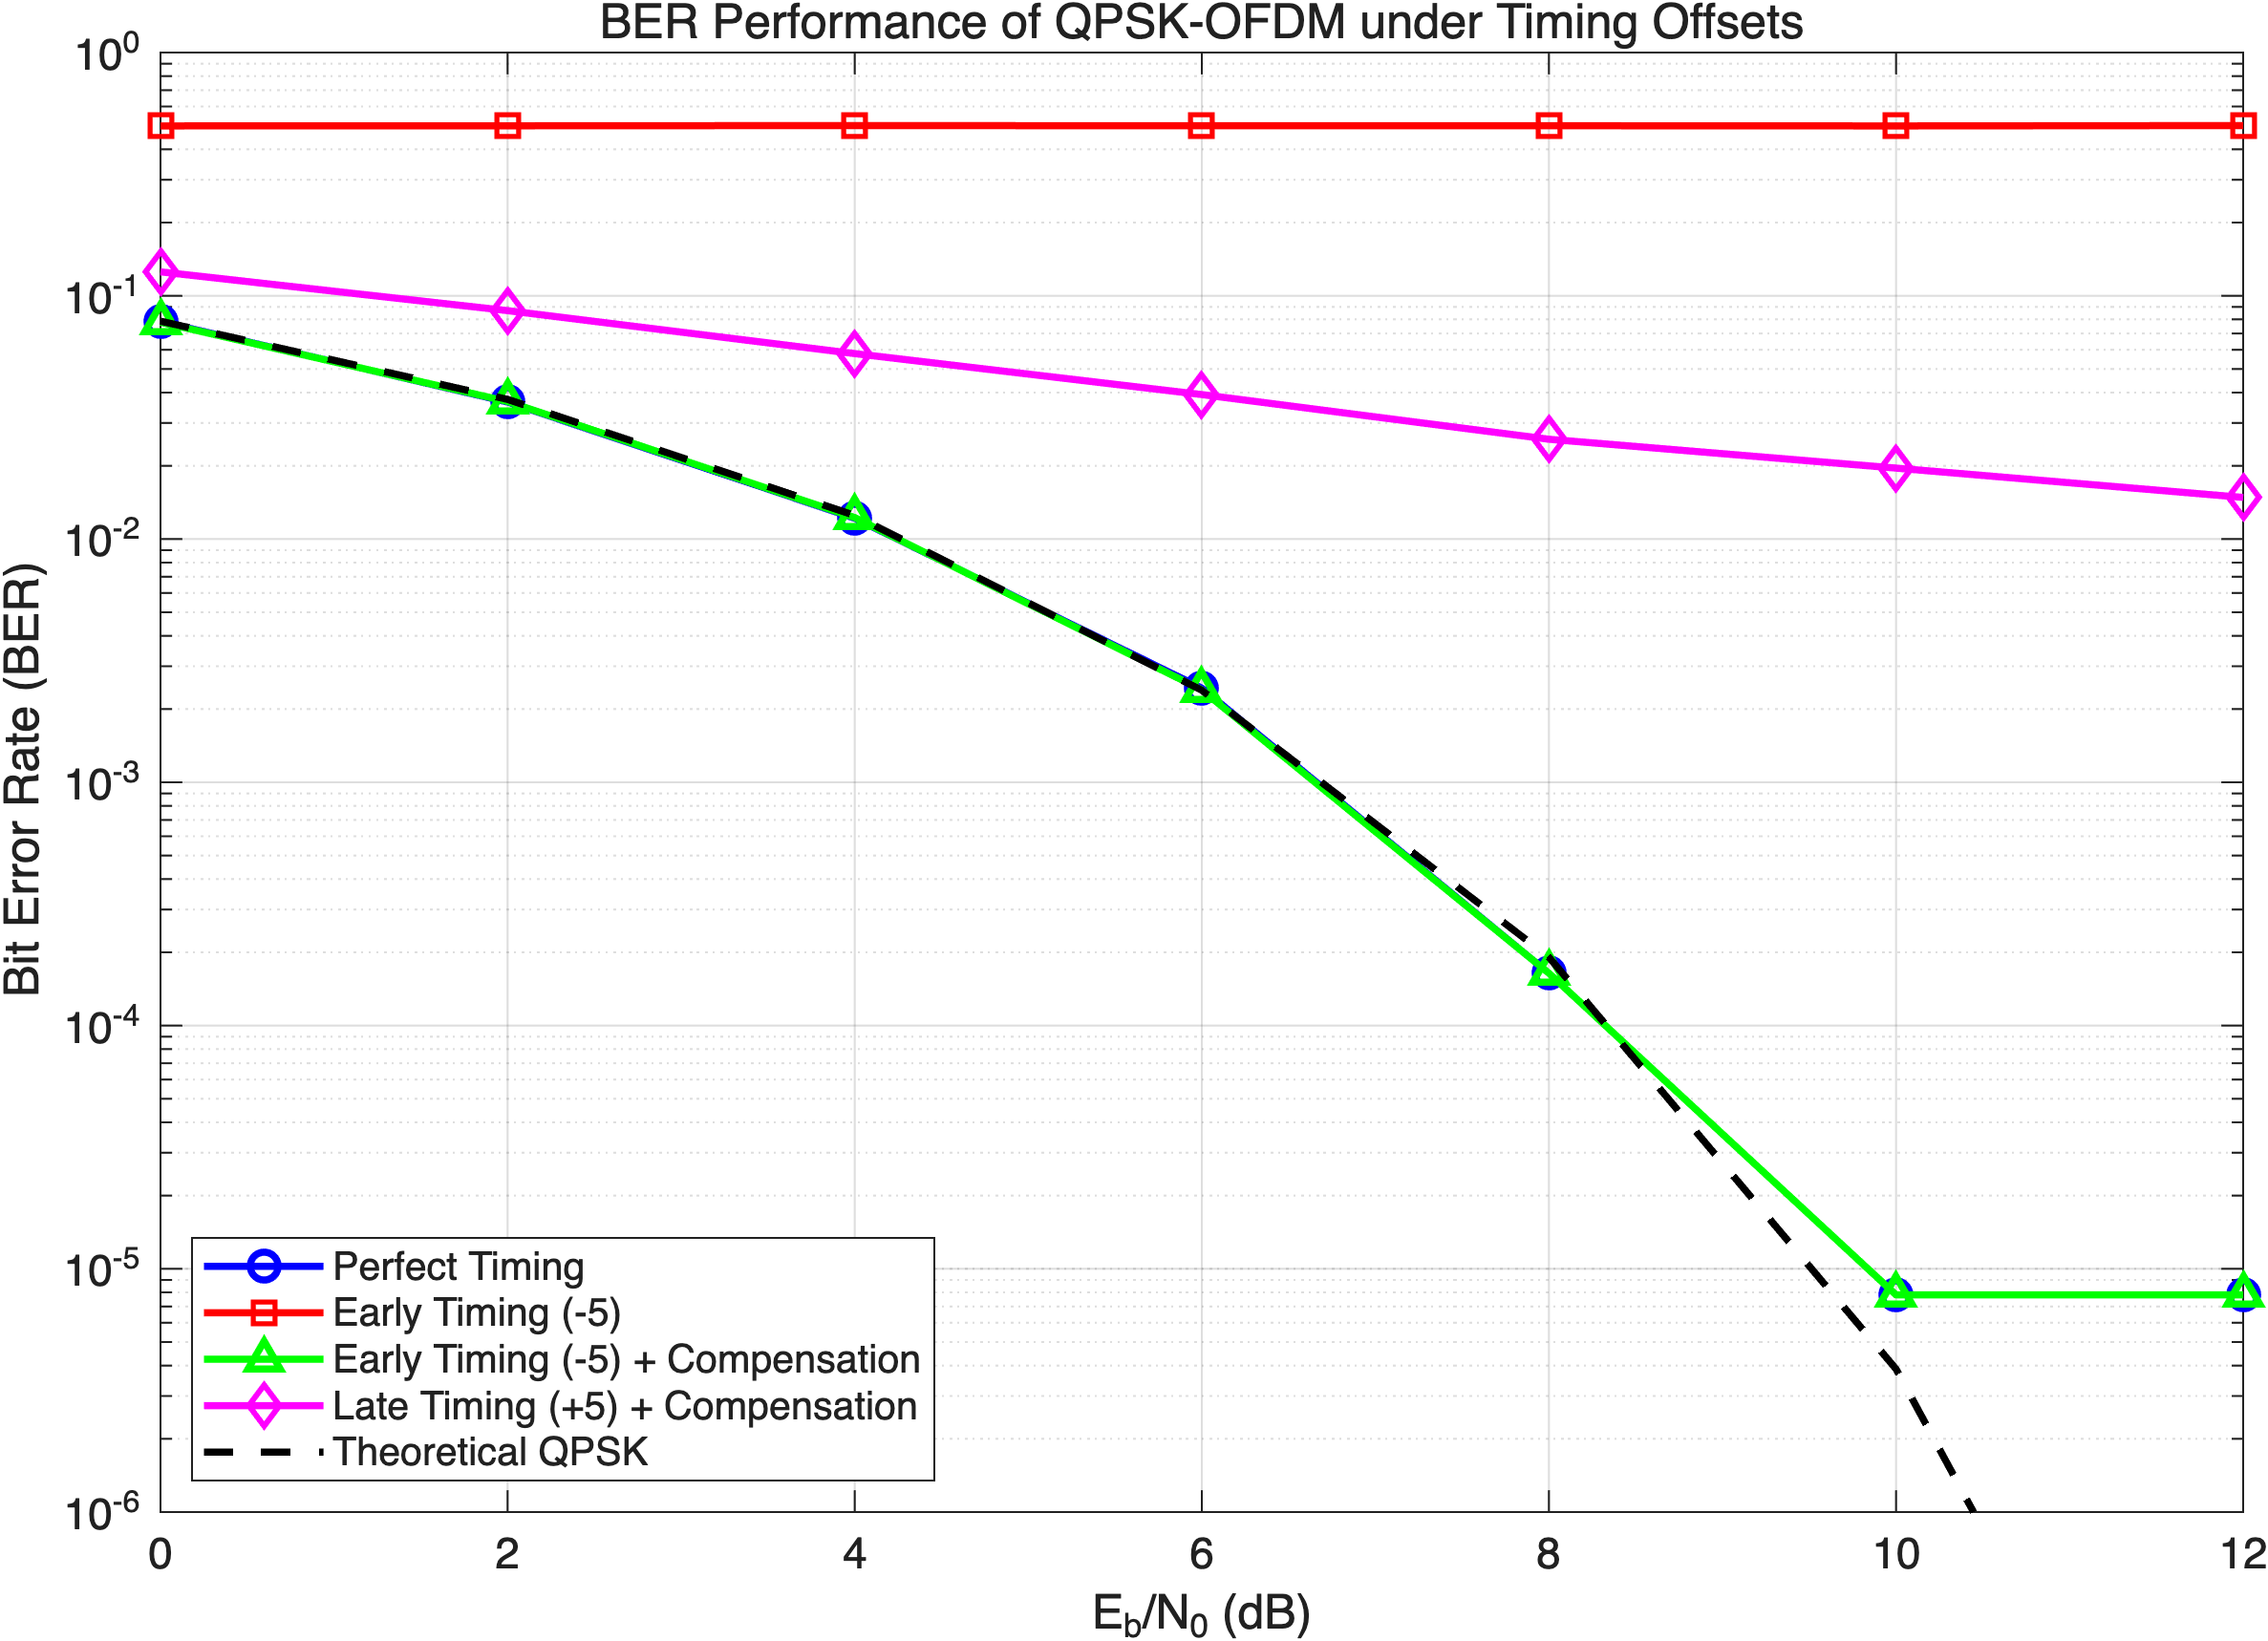
\includegraphics[width=.88\linewidth]{figures/ch4/exp02_ber_vs_ebn0.png}
\caption{EXP02: BER under AWGN with imposed timing offsets. Observed zero BER values are displayed at $1/128000$ for logarithmic plotting only.}
\label{fig:ch4_offset_snr}
\end{figure}

\section[Individual Estimator Checks]{Individual Estimator Validation}
\label{sec:ch4_individual}
EXP03--06 establish that the implemented timing metrics and decision rules operate before the formal comparison. These experiments are not used to rank the four methods because the earlier search settings and random scenarios are not identical.

In the noiseless S\&C verification (EXP03), the arrival delay is 50 samples and the true useful start is 67 in MATLAB indexing. The metric remains at one from candidate 51 to 67 inclusive, a plateau covering the CP and the true start. Figure~\ref{fig:ch4_plateau} shows this ambiguity. The individual AWGN Monte Carlo experiment records an exact probability of 0.0010 but a CP-safe probability of 0.9999 at 20 dB. These values already indicate that low noise does not remove the systematic displacement caused by a plateau-midpoint decision.

\begin{figure}[!htbp]
\centering
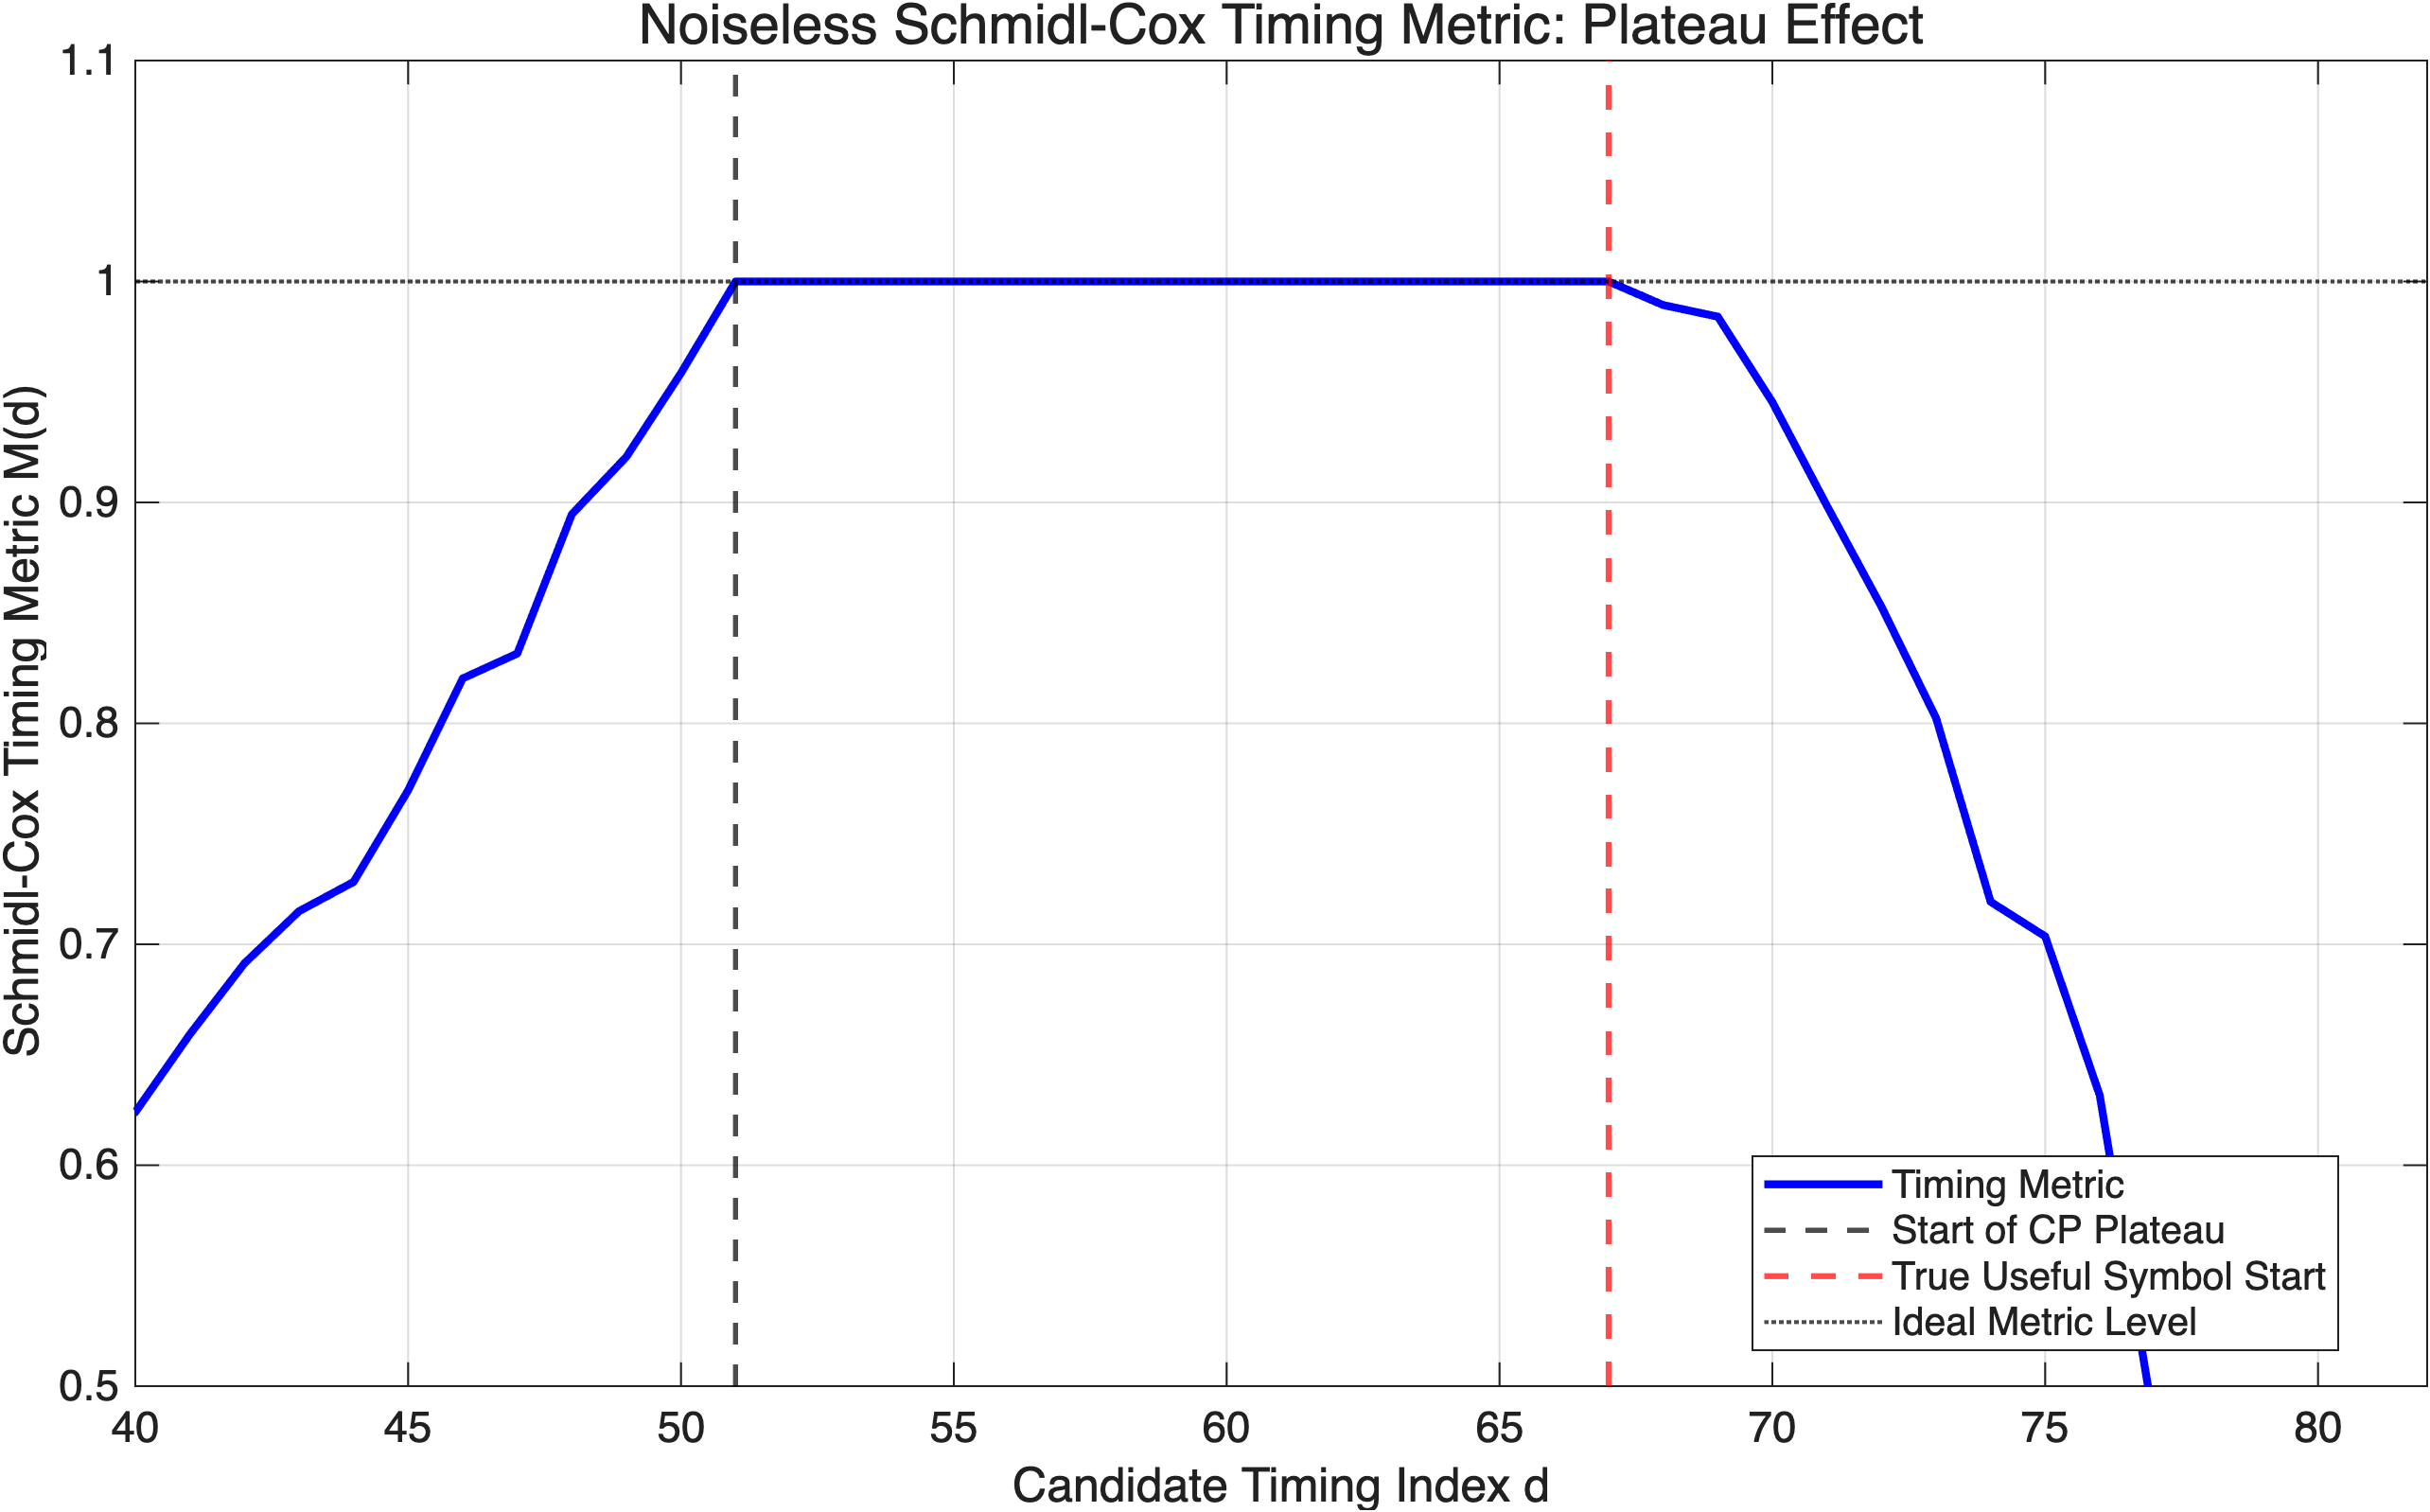
\includegraphics[width=.88\linewidth]{figures/ch4/sc_noiseless_timing_metric_zoom.png}
\caption{EXP03: noiseless S\&C plateau, with the CP start at 51 and useful-symbol start at 67.}
\label{fig:ch4_plateau}
\end{figure}

The final Park-type experiment (EXP04) records exact probabilities of 0.9184 in AWGN and 0.5442 in the fixed multipath channel at 0 dB. By 10 dB these become 1.0000 and 0.9895. Earlier Park structure and normalization diagnostics are not substituted for the final supervisor-confirmed version. In EXP05, the Minn-type estimator gives exact probabilities of 0.6153 and 0.4564 in AWGN and multipath at 0 dB, rising to 0.9991 and 0.9957 at 10 dB. In EXP06, CAZAC records exact probability 1.0000 throughout the AWGN grid and 0.9996 at 0 dB in the fixed multipath channel. These checks motivate the unified comparison; their numerical values should not be pooled with EXP07 results.

\section[Unified Timing Metrics]{Timing Metric Examples in EXP07}
\label{sec:ch4_metrics}
The representative metric experiment uses a fixed arrival delay $D=50$ and maps each algorithm's candidate indices to the common useful-start coordinate. The true useful training start is 67. The horizontal axes in Figures~\ref{fig:ch4_metric_ideal}--\ref{fig:ch4_metric_mp} show candidate error relative to this start. Each curve is normalized for display; these plotted heights must not be interpreted as identically calibrated decision metrics. The actual estimates are obtained from the algorithms and eligibility conditions specified in Chapter 3.

\begin{figure}[!htbp]
\centering
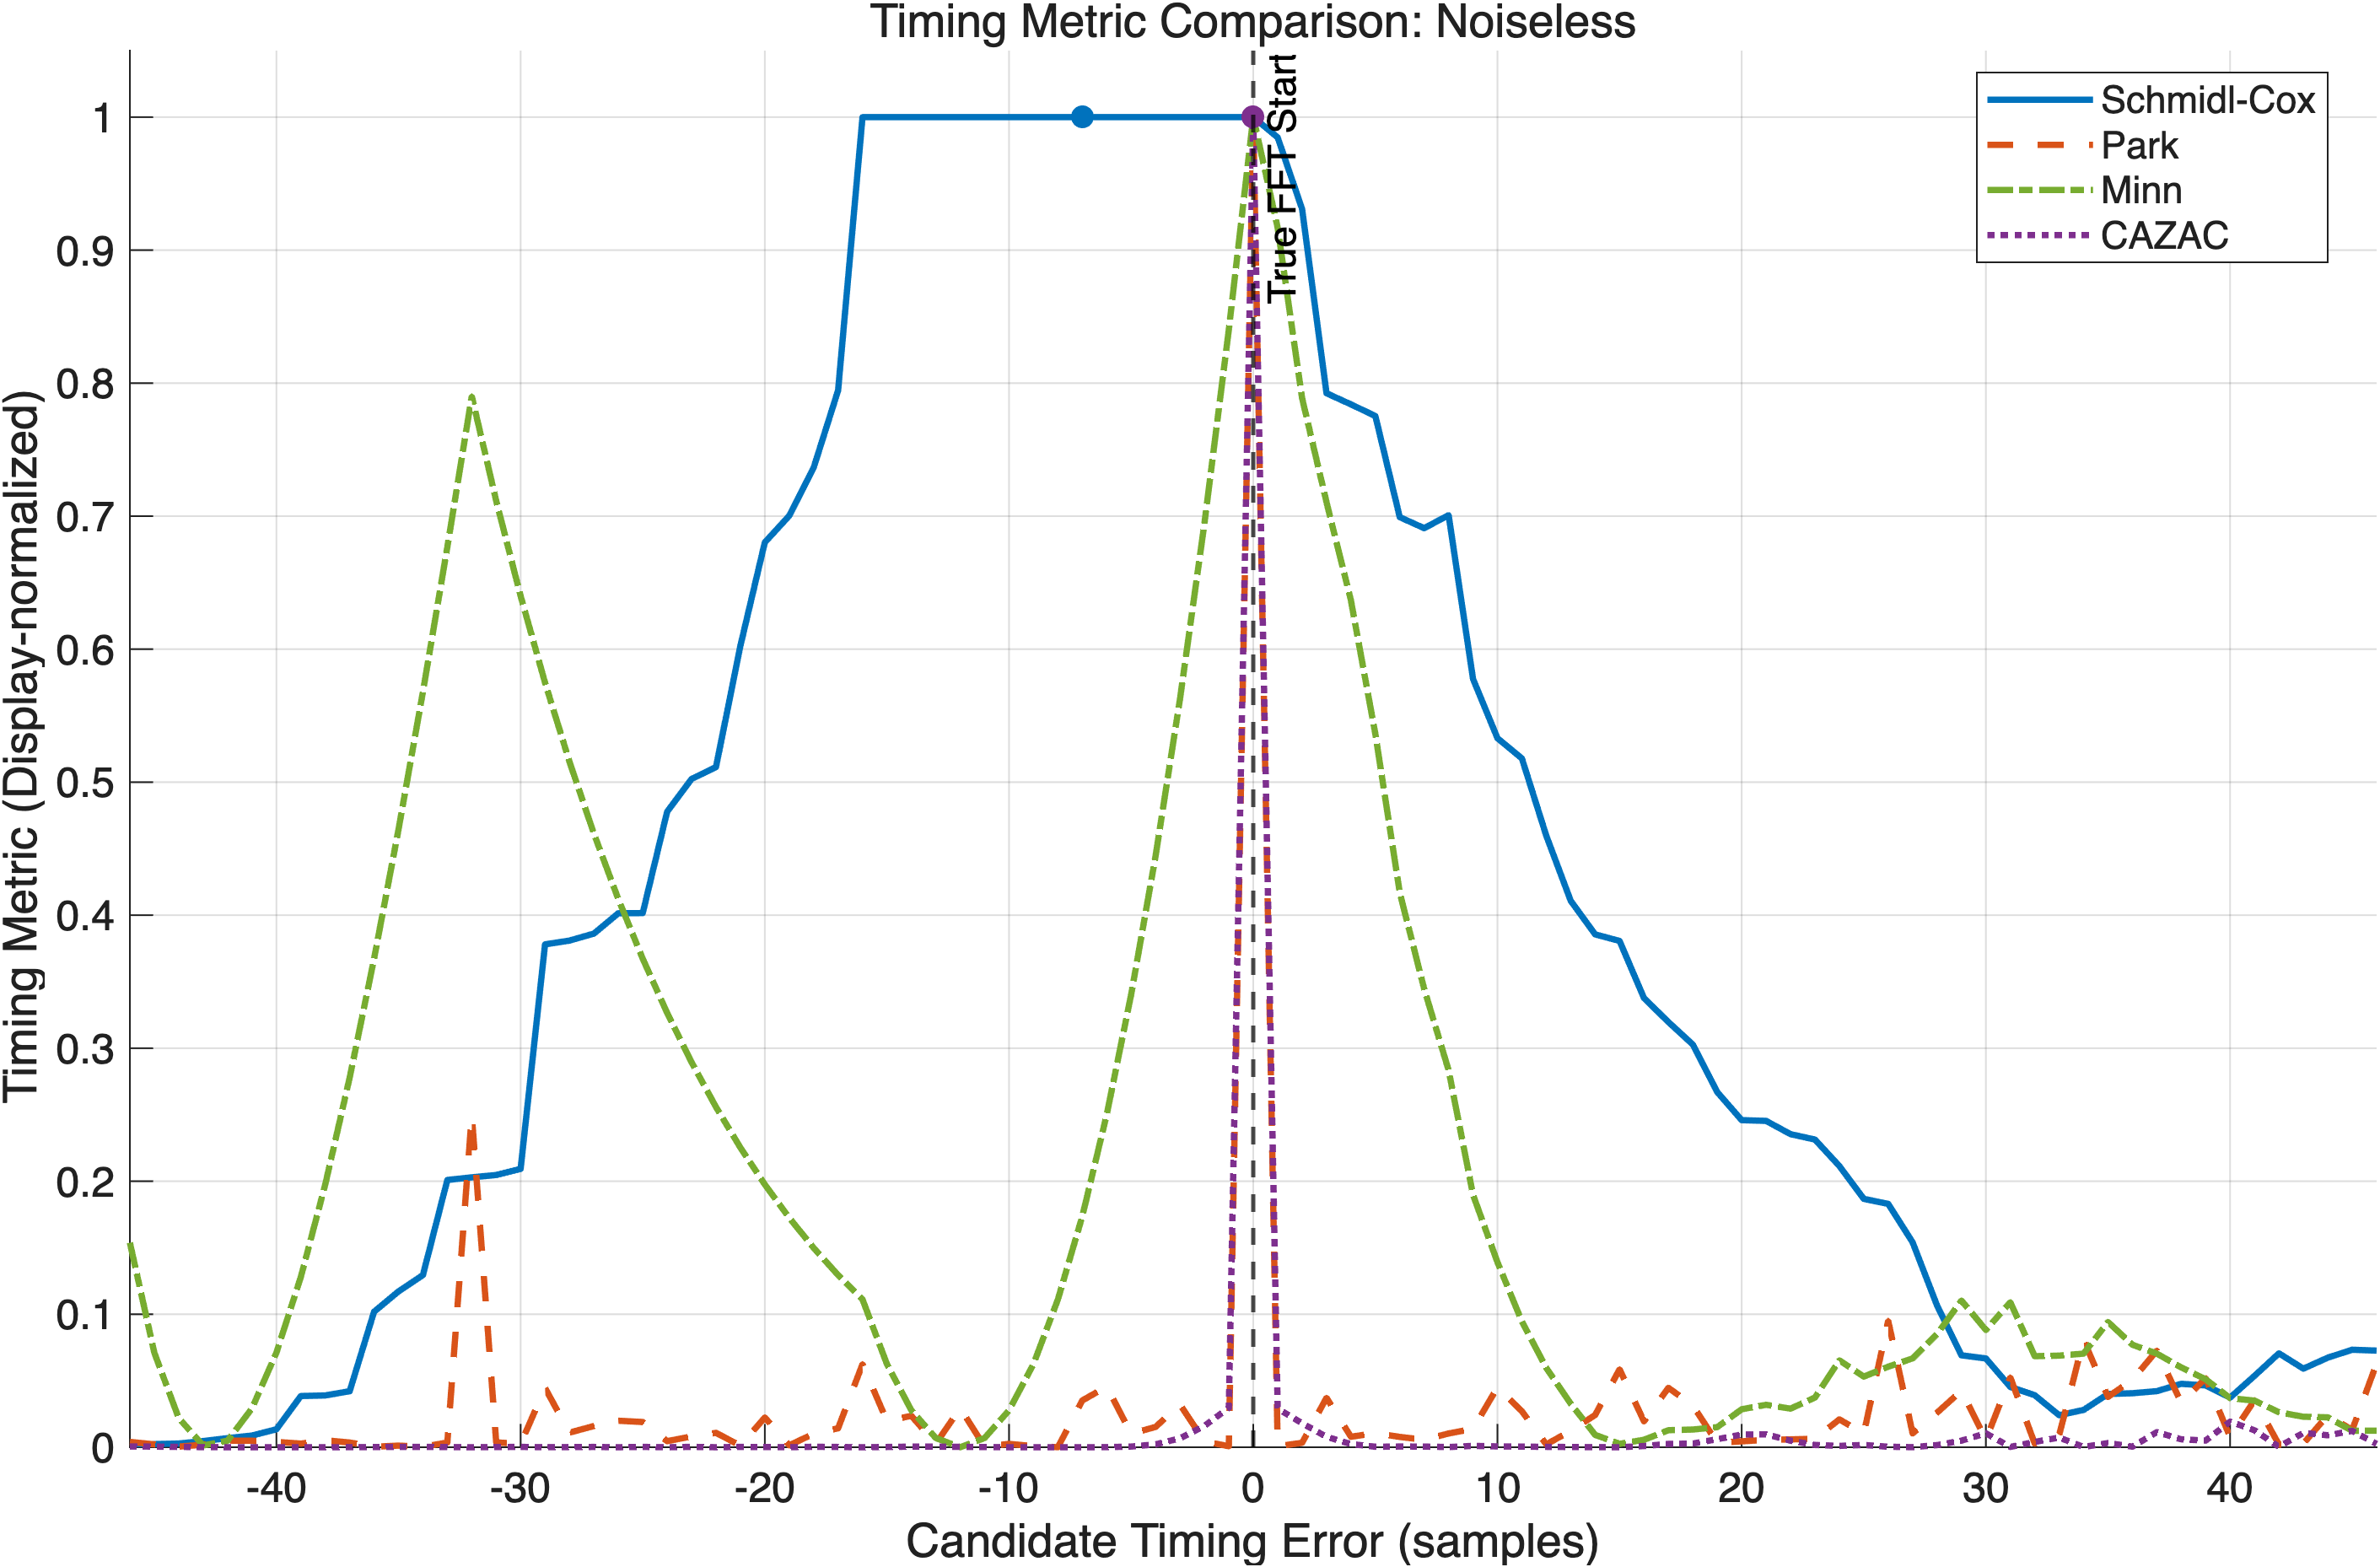
\includegraphics[width=.88\linewidth]{figures/ch4/exp07_metric_noiseless.png}
\caption{EXP07: display-normalized timing metrics in the noiseless single-path case.}
\label{fig:ch4_metric_ideal}
\end{figure}

\begin{figure}[!htbp]
\centering
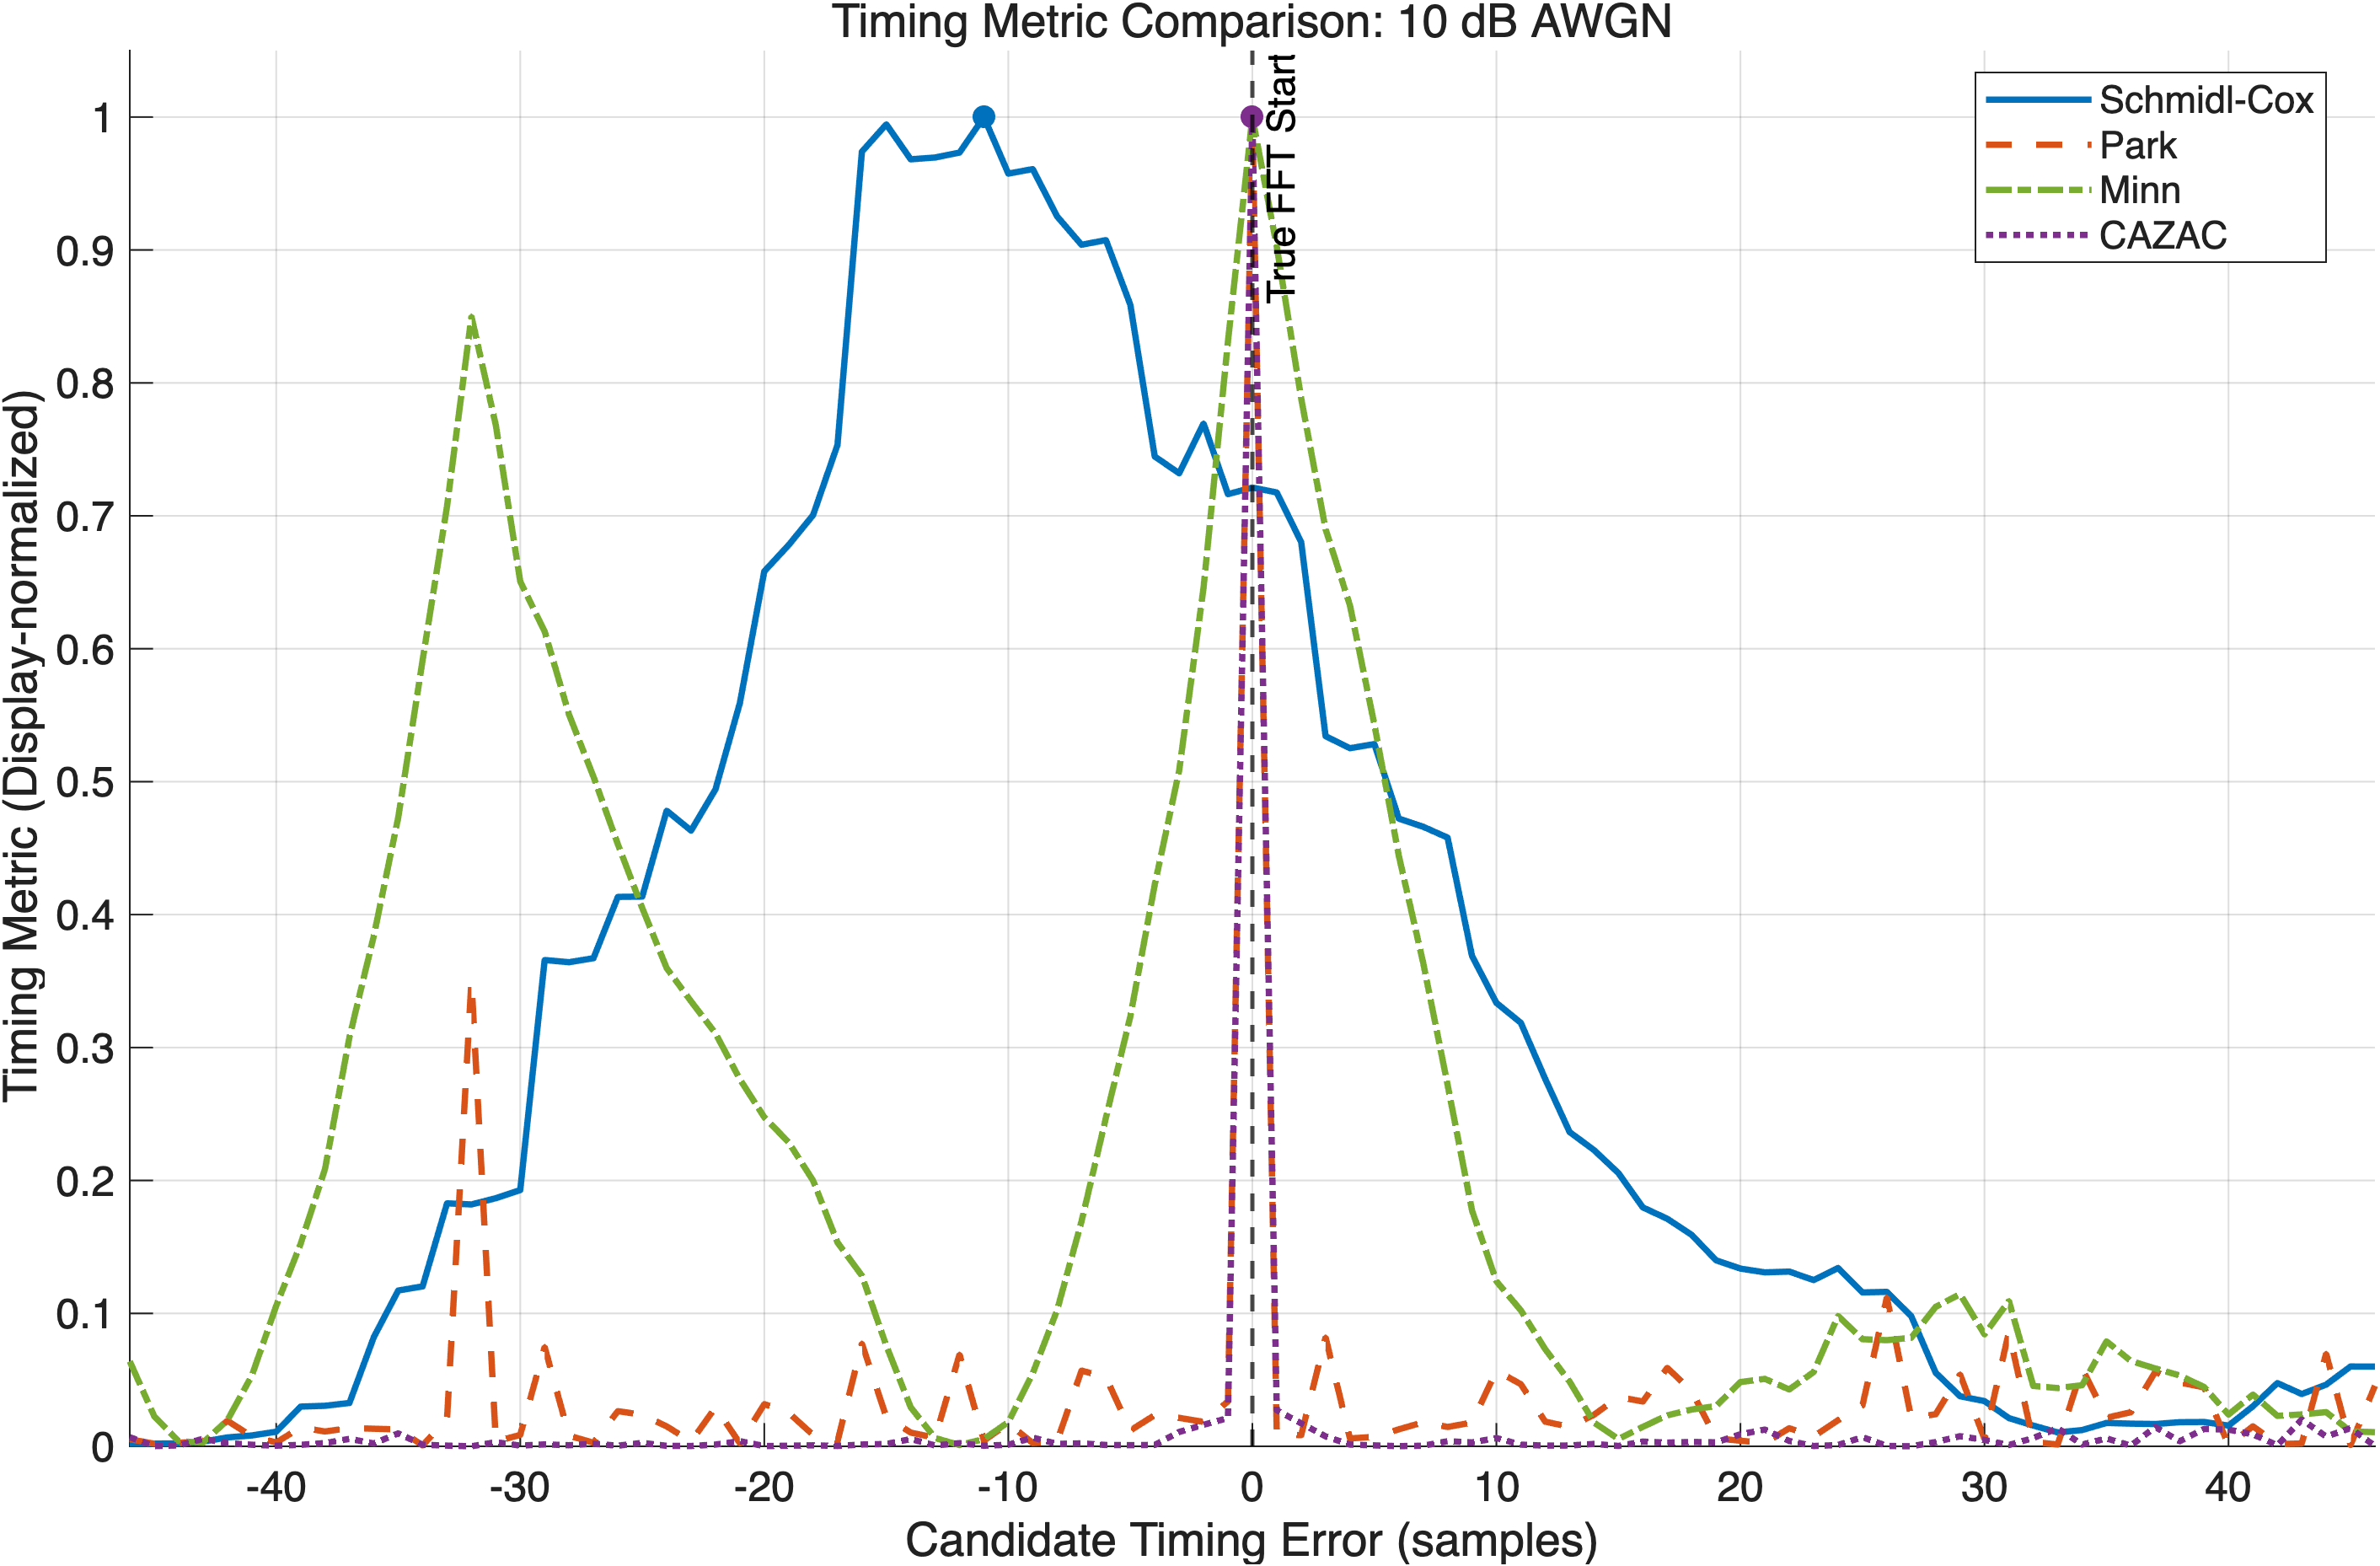
\includegraphics[width=.88\linewidth]{figures/ch4/exp07_metric_awgn_10dB.png}
\caption{EXP07: representative display-normalized timing metrics at 10 dB AWGN.}
\label{fig:ch4_metric_awgn}
\end{figure}

\begin{figure}[!htbp]
\centering
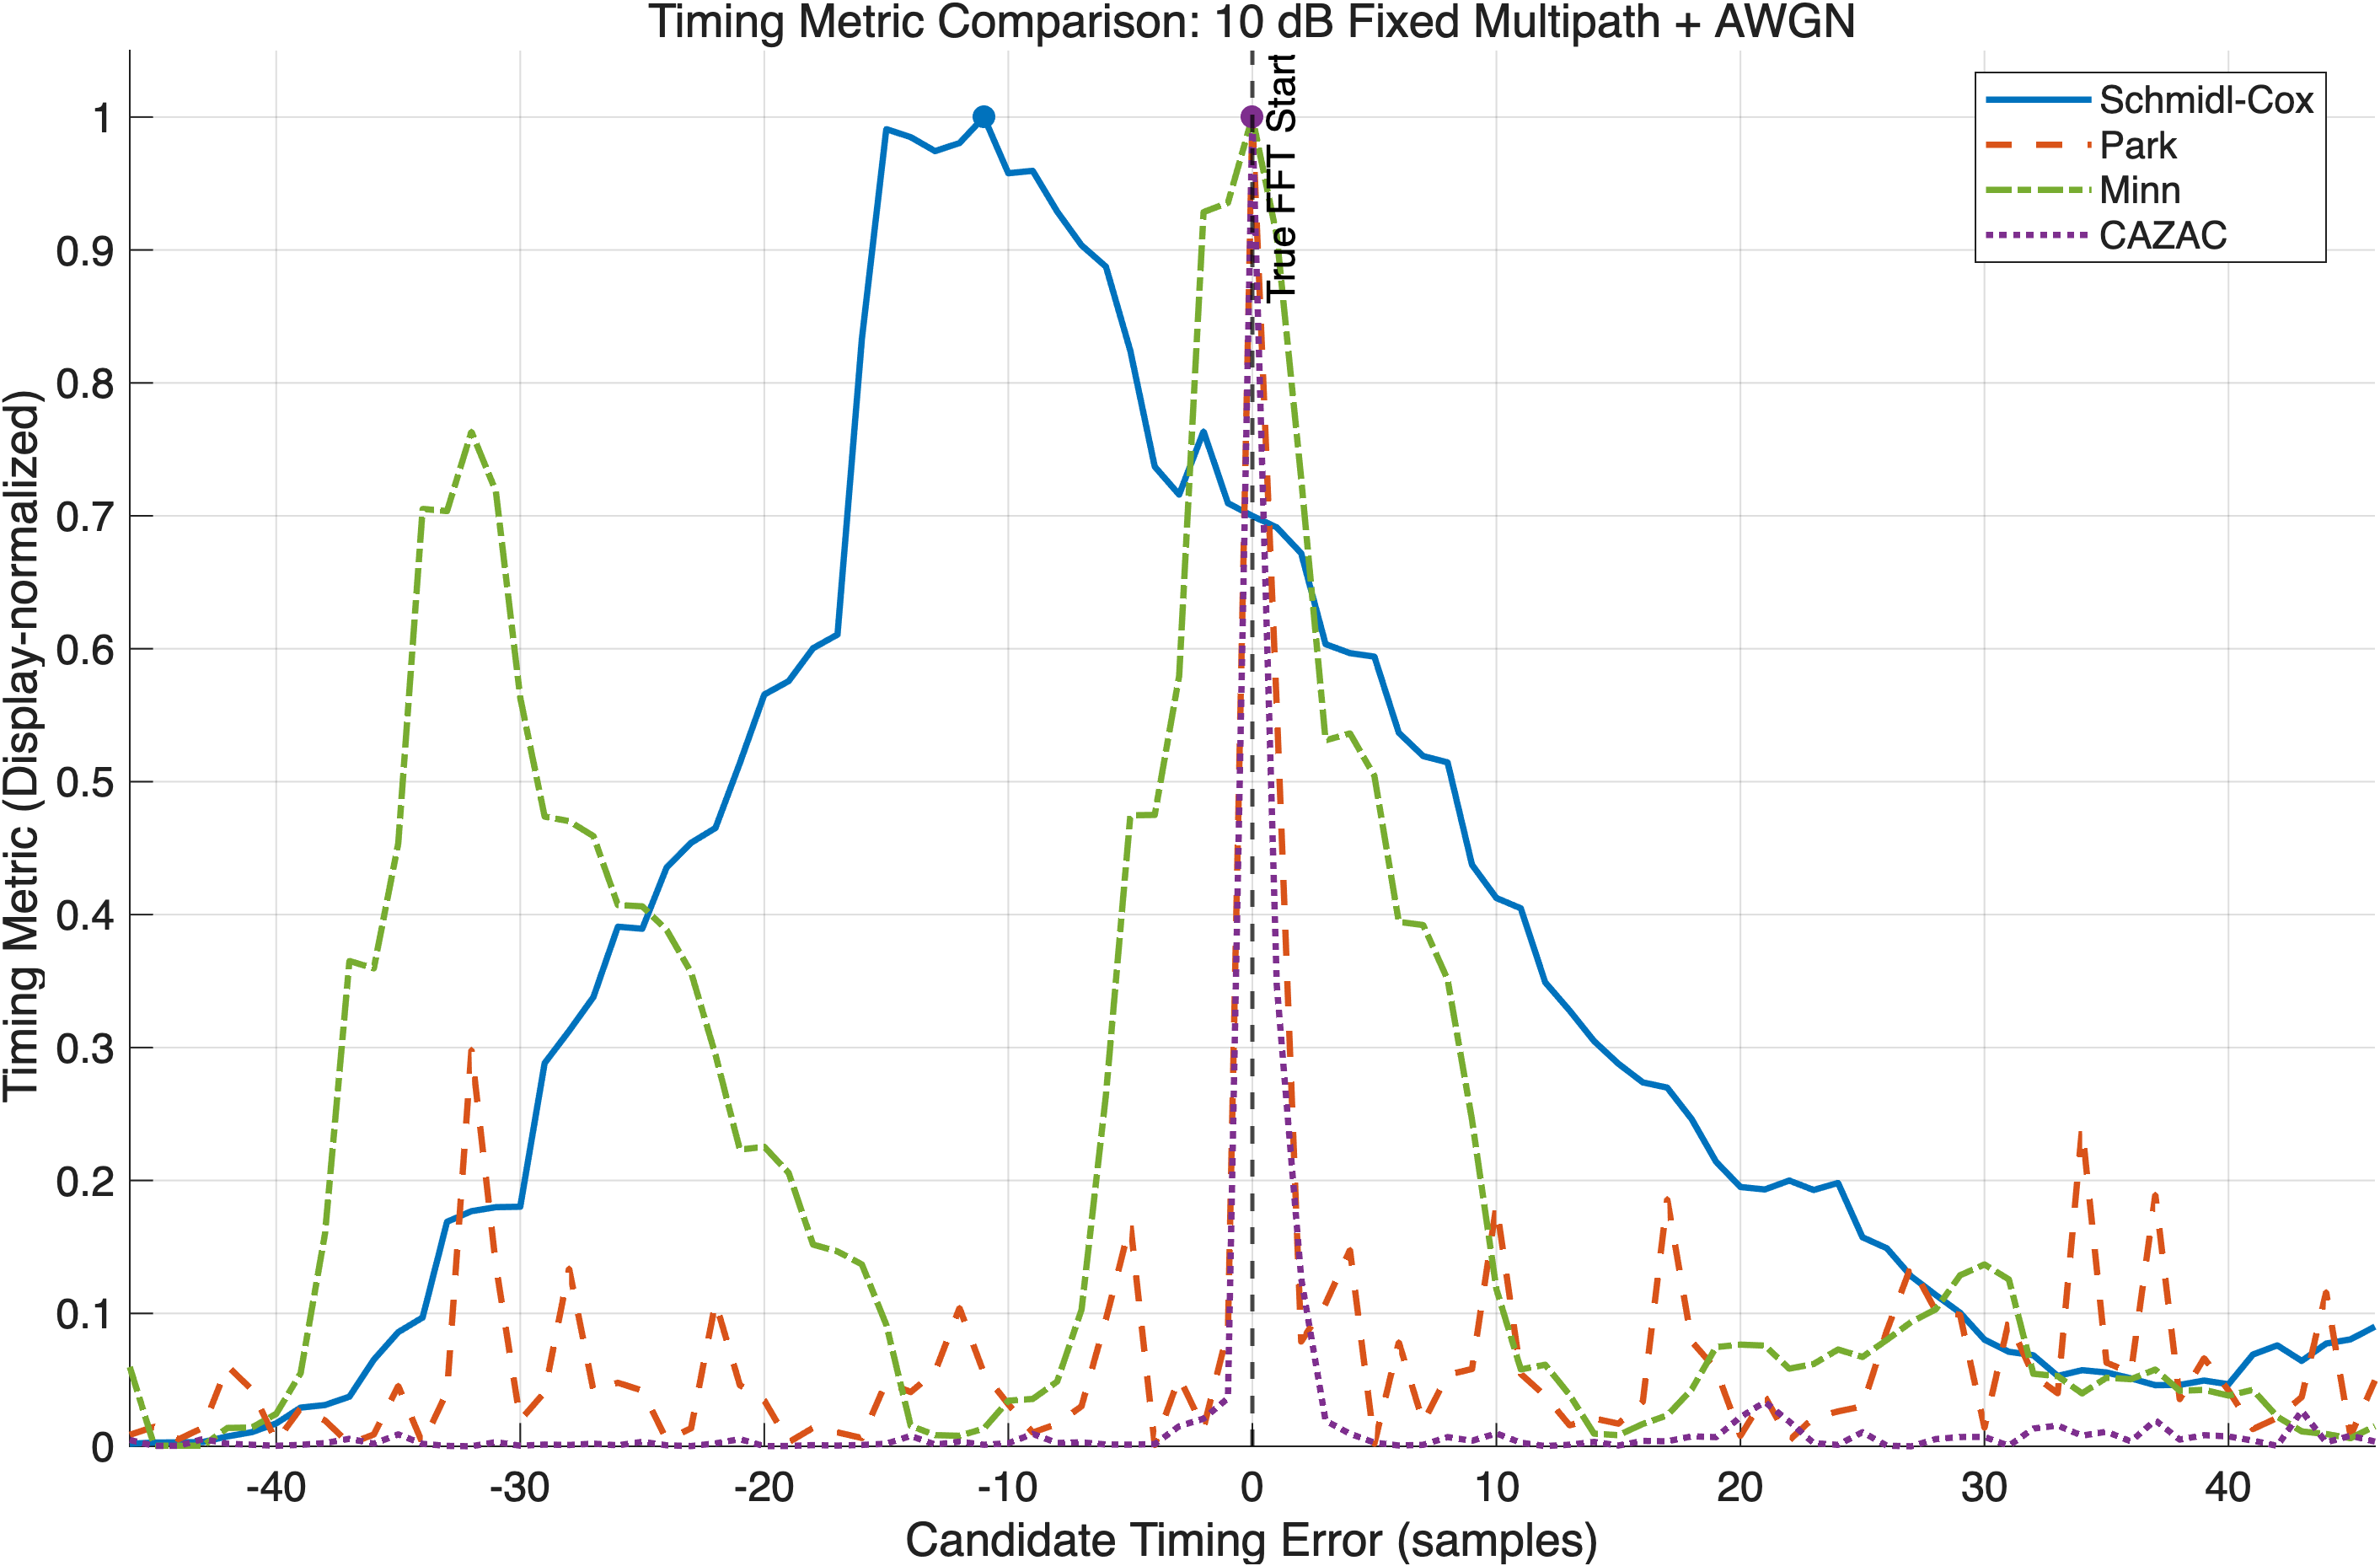
\includegraphics[width=.88\linewidth]{figures/ch4/exp07_metric_multipath_10dB.png}
\caption{EXP07: representative display-normalized timing metrics at 10 dB in fixed multipath.}
\label{fig:ch4_metric_mp}
\end{figure}

\begin{table}[htbp]
\centering
\caption{Timing errors in the three representative EXP07 frames (samples).}
\label{tab:ch4_examples}
\begin{tabular}{lrrrr}
\hline
Scenario & S\&C & Park & Minn & CAZAC\\
\hline
Noiseless & $-7$ & 0 & 0 & 0\\
AWGN, 10 dB & $-11$ & 0 & 0 & 0\\
Multipath, 10 dB & $-11$ & 0 & 0 & 0\\
\hline
\end{tabular}
\end{table}
The S\&C curve displays a broad plateau or rounded high-metric region; the three other methods provide a more localized maximum near the reference in these particular observations. Minn also exhibits a competing peak approximately 32 samples before the useful start, consistent with its signed-block structure. The Park metric is affected by local symmetry and multipath, while CAZAC uses the complete known template. Table~\ref{tab:ch4_examples} reports the actual decisions. The three peak-based methods return the true start in all three displayed frames; S\&C selects an early position. A single representative observation cannot establish the probability of choosing a competing peak, so statistical comparison is required.

\section[Unified Monte Carlo Results]{Unified Monte Carlo Timing Results}
\label{sec:ch4_comparison}
EXP07 contains 10,000 estimates for every algorithm, SNR and channel combination, giving 880,000 attempted timing estimates. All are valid, and all 88 condition-level summaries have zero observed no-estimate events. This is not a claim that every estimate is correct or that a noise-only frame would be rejected. Tables~\ref{tab:ch4_awgn} and~\ref{tab:ch4_mp} report representative SNR levels; Figures~\ref{fig:ch4_mse}--\ref{fig:ch4_cpsafe} show the full grid. Since no estimate is invalid, the conditional MSE equals the empirical MSE over all 10,000 attempts in each condition.

\begin{table}[htbp]
\centering
\caption{EXP07 timing performance in AWGN at selected SNRs. MSE is in samples squared.}
\label{tab:ch4_awgn}
\small
\begin{tabular}{rlrrr}
\hline
SNR (dB) & Method & Exact & CP-safe & MSE\\
\hline
0 & S\&C & 0.0576 & 0.6773 & 135.9962 \\
 & Park & 0.8981 & 0.9132 & 100.1021 \\
 & Minn & 0.6438 & 0.7384 & 116.1906 \\
 & CAZAC & 1.0000 & 1.0000 & 0.0000 \\
\hline
10 & S\&C & 0.0385 & 0.9501 & 81.6839 \\
 & Park & 1.0000 & 1.0000 & 0.0000 \\
 & Minn & 0.9989 & 0.9989 & 0.9218 \\
 & CAZAC & 1.0000 & 1.0000 & 0.0000 \\
\hline
20 & S\&C & 0.0006 & 0.9978 & 59.4513 \\
 & Park & 1.0000 & 1.0000 & 0.0000 \\
 & Minn & 1.0000 & 1.0000 & 0.0000 \\
 & CAZAC & 1.0000 & 1.0000 & 0.0000 \\
\hline
\end{tabular}
\end{table}

\begin{table}[htbp]
\centering
\caption{EXP07 timing performance in fixed multipath with AWGN at selected SNRs. MSE is in samples squared.}
\label{tab:ch4_mp}
\small
\begin{tabular}{rlrrr}
\hline
SNR (dB) & Method & Exact & CP-safe & MSE\\
\hline
0 & S\&C & 0.0561 & 0.5611 & 136.6196 \\
 & Park & 0.4856 & 0.5363 & 322.0781 \\
 & Minn & 0.4653 & 0.7605 & 96.4519 \\
 & CAZAC & 0.9998 & 0.9998 & 0.0002 \\
\hline
10 & S\&C & 0.0393 & 0.8753 & 76.9561 \\
 & Park & 0.9902 & 0.9905 & 0.8639 \\
 & Minn & 0.9955 & 0.9998 & 0.1140 \\
 & CAZAC & 1.0000 & 1.0000 & 0.0000 \\
\hline
20 & S\&C & 0.0013 & 0.9924 & 55.6819 \\
 & Park & 0.9999 & 0.9999 & 0.0361 \\
 & Minn & 1.0000 & 1.0000 & 0.0000 \\
 & CAZAC & 1.0000 & 1.0000 & 0.0000 \\
\hline
\end{tabular}
\end{table}

\begin{figure}[p]
\centering
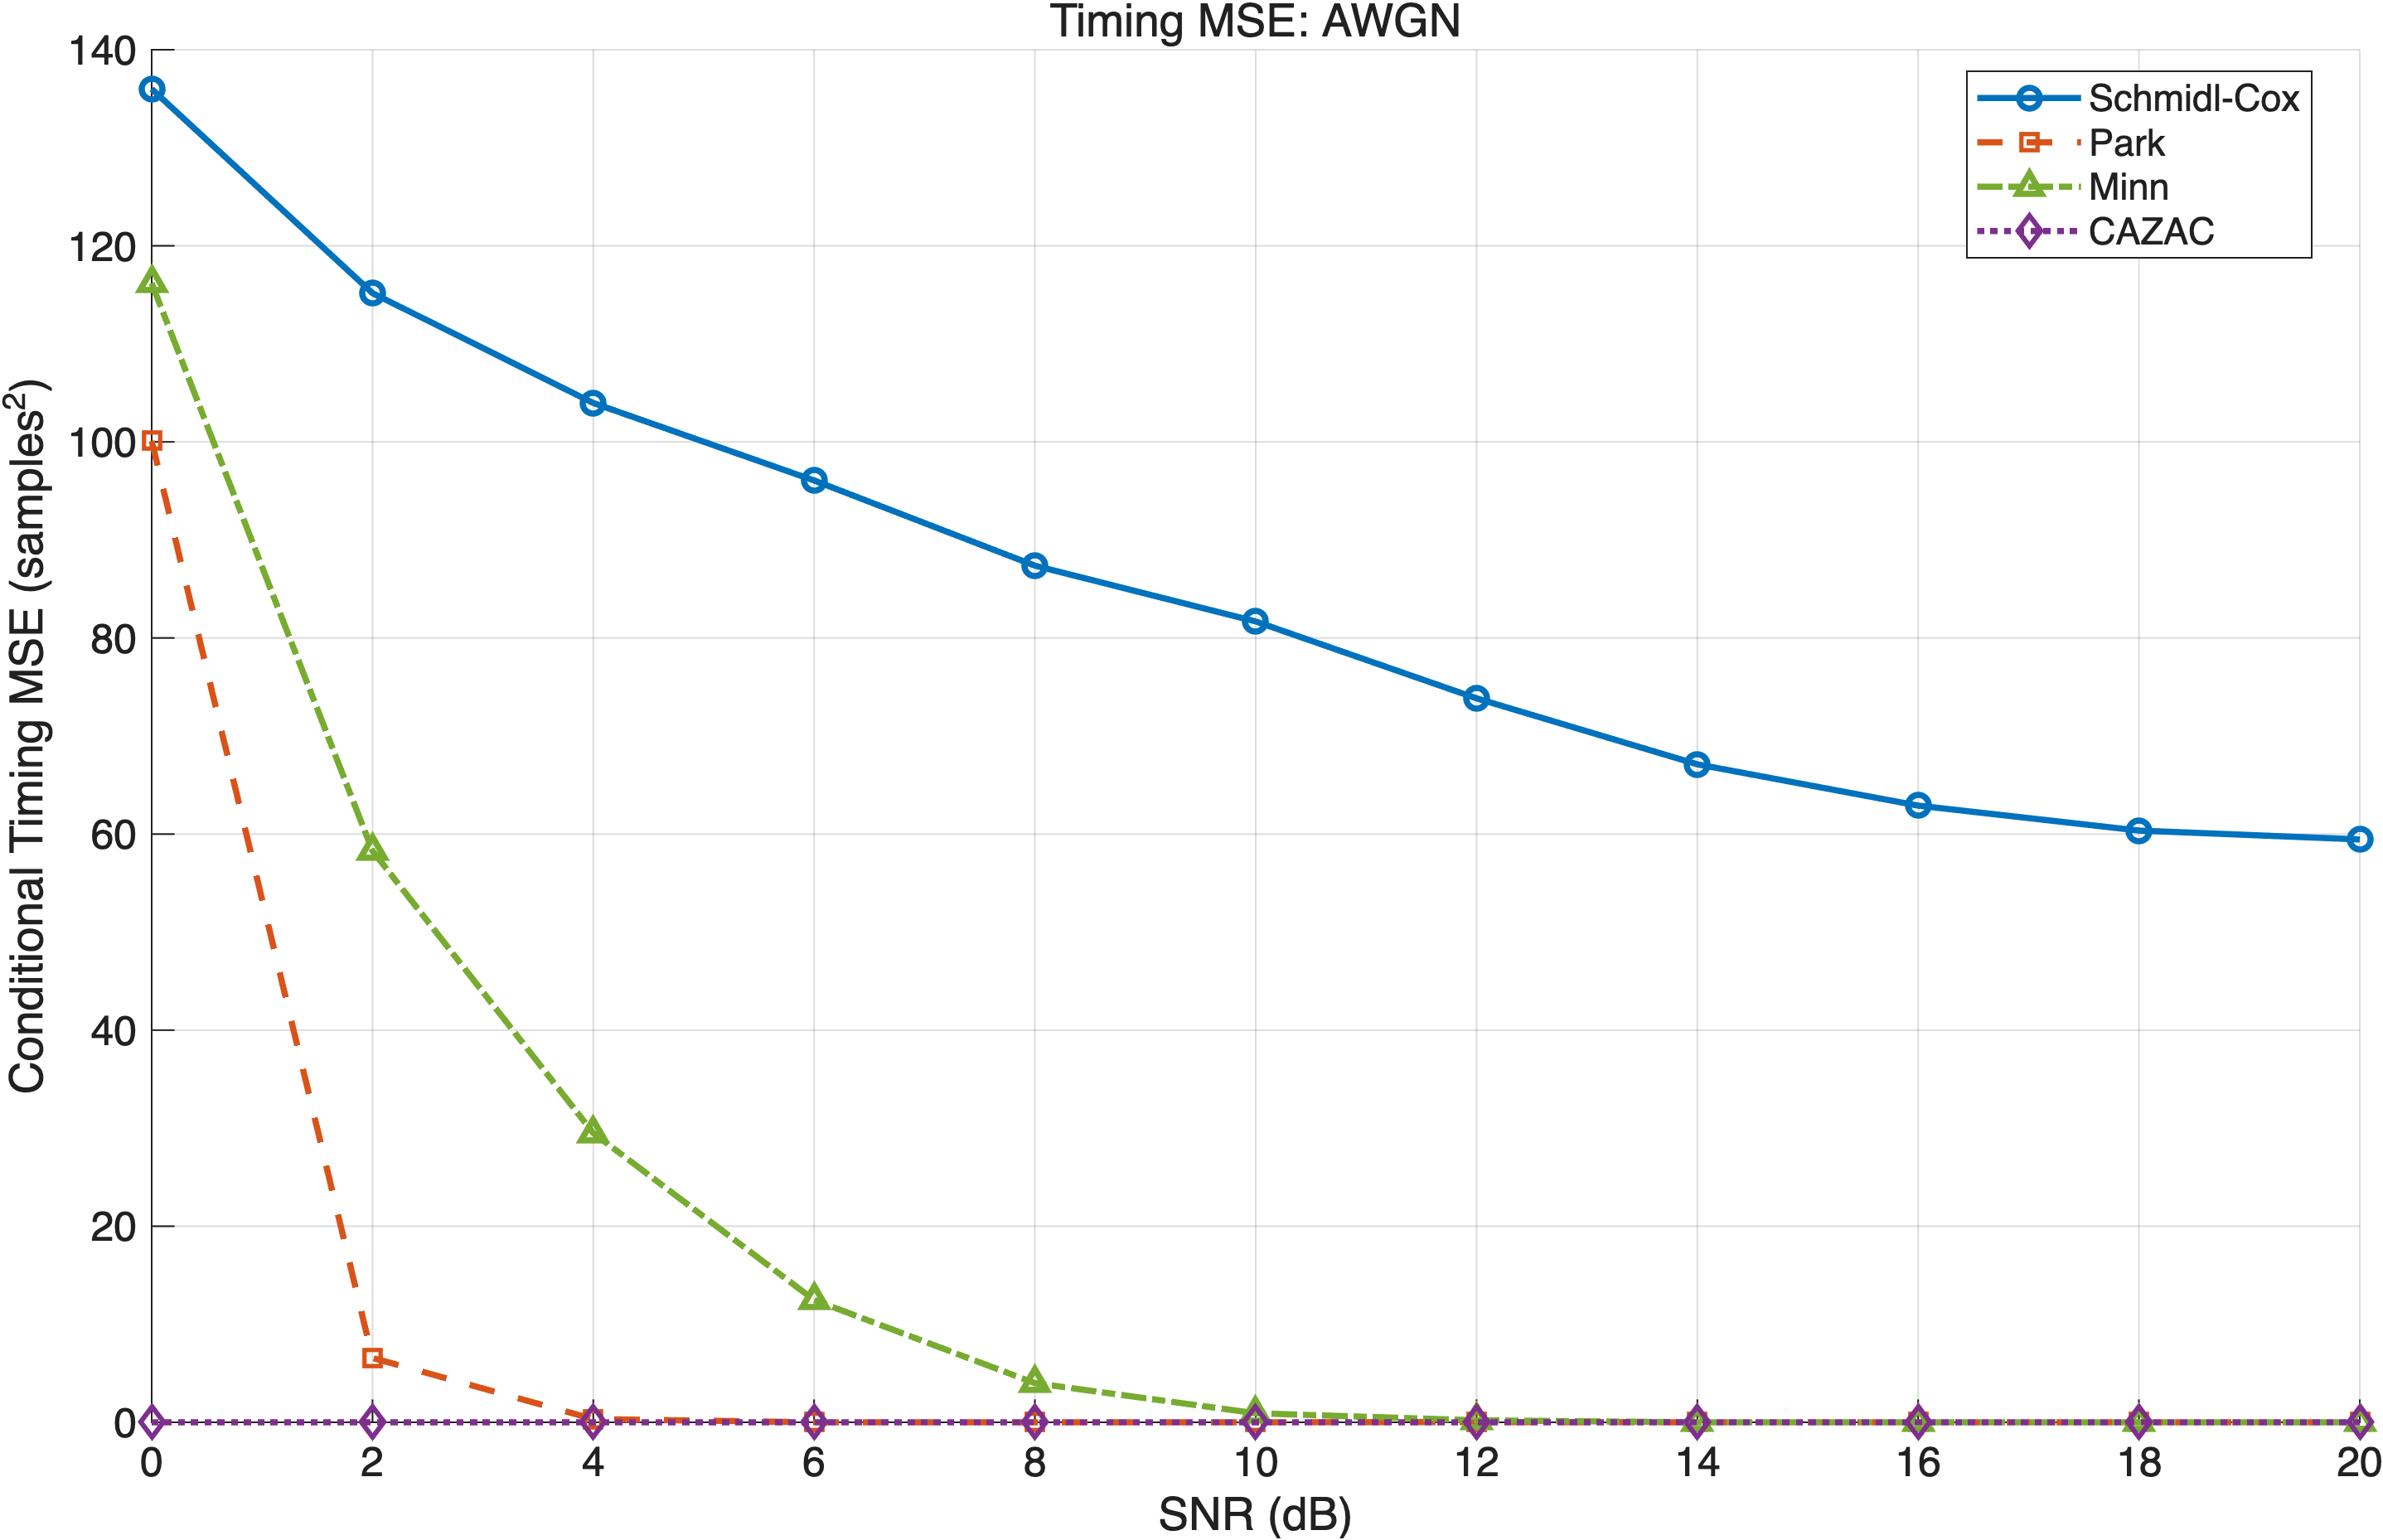
\includegraphics[width=0.84\linewidth,height=0.36\textheight,keepaspectratio]{figures/ch4/exp07_awgn_mse.png}\par\smallskip
{\small (a) AWGN}\par\medskip
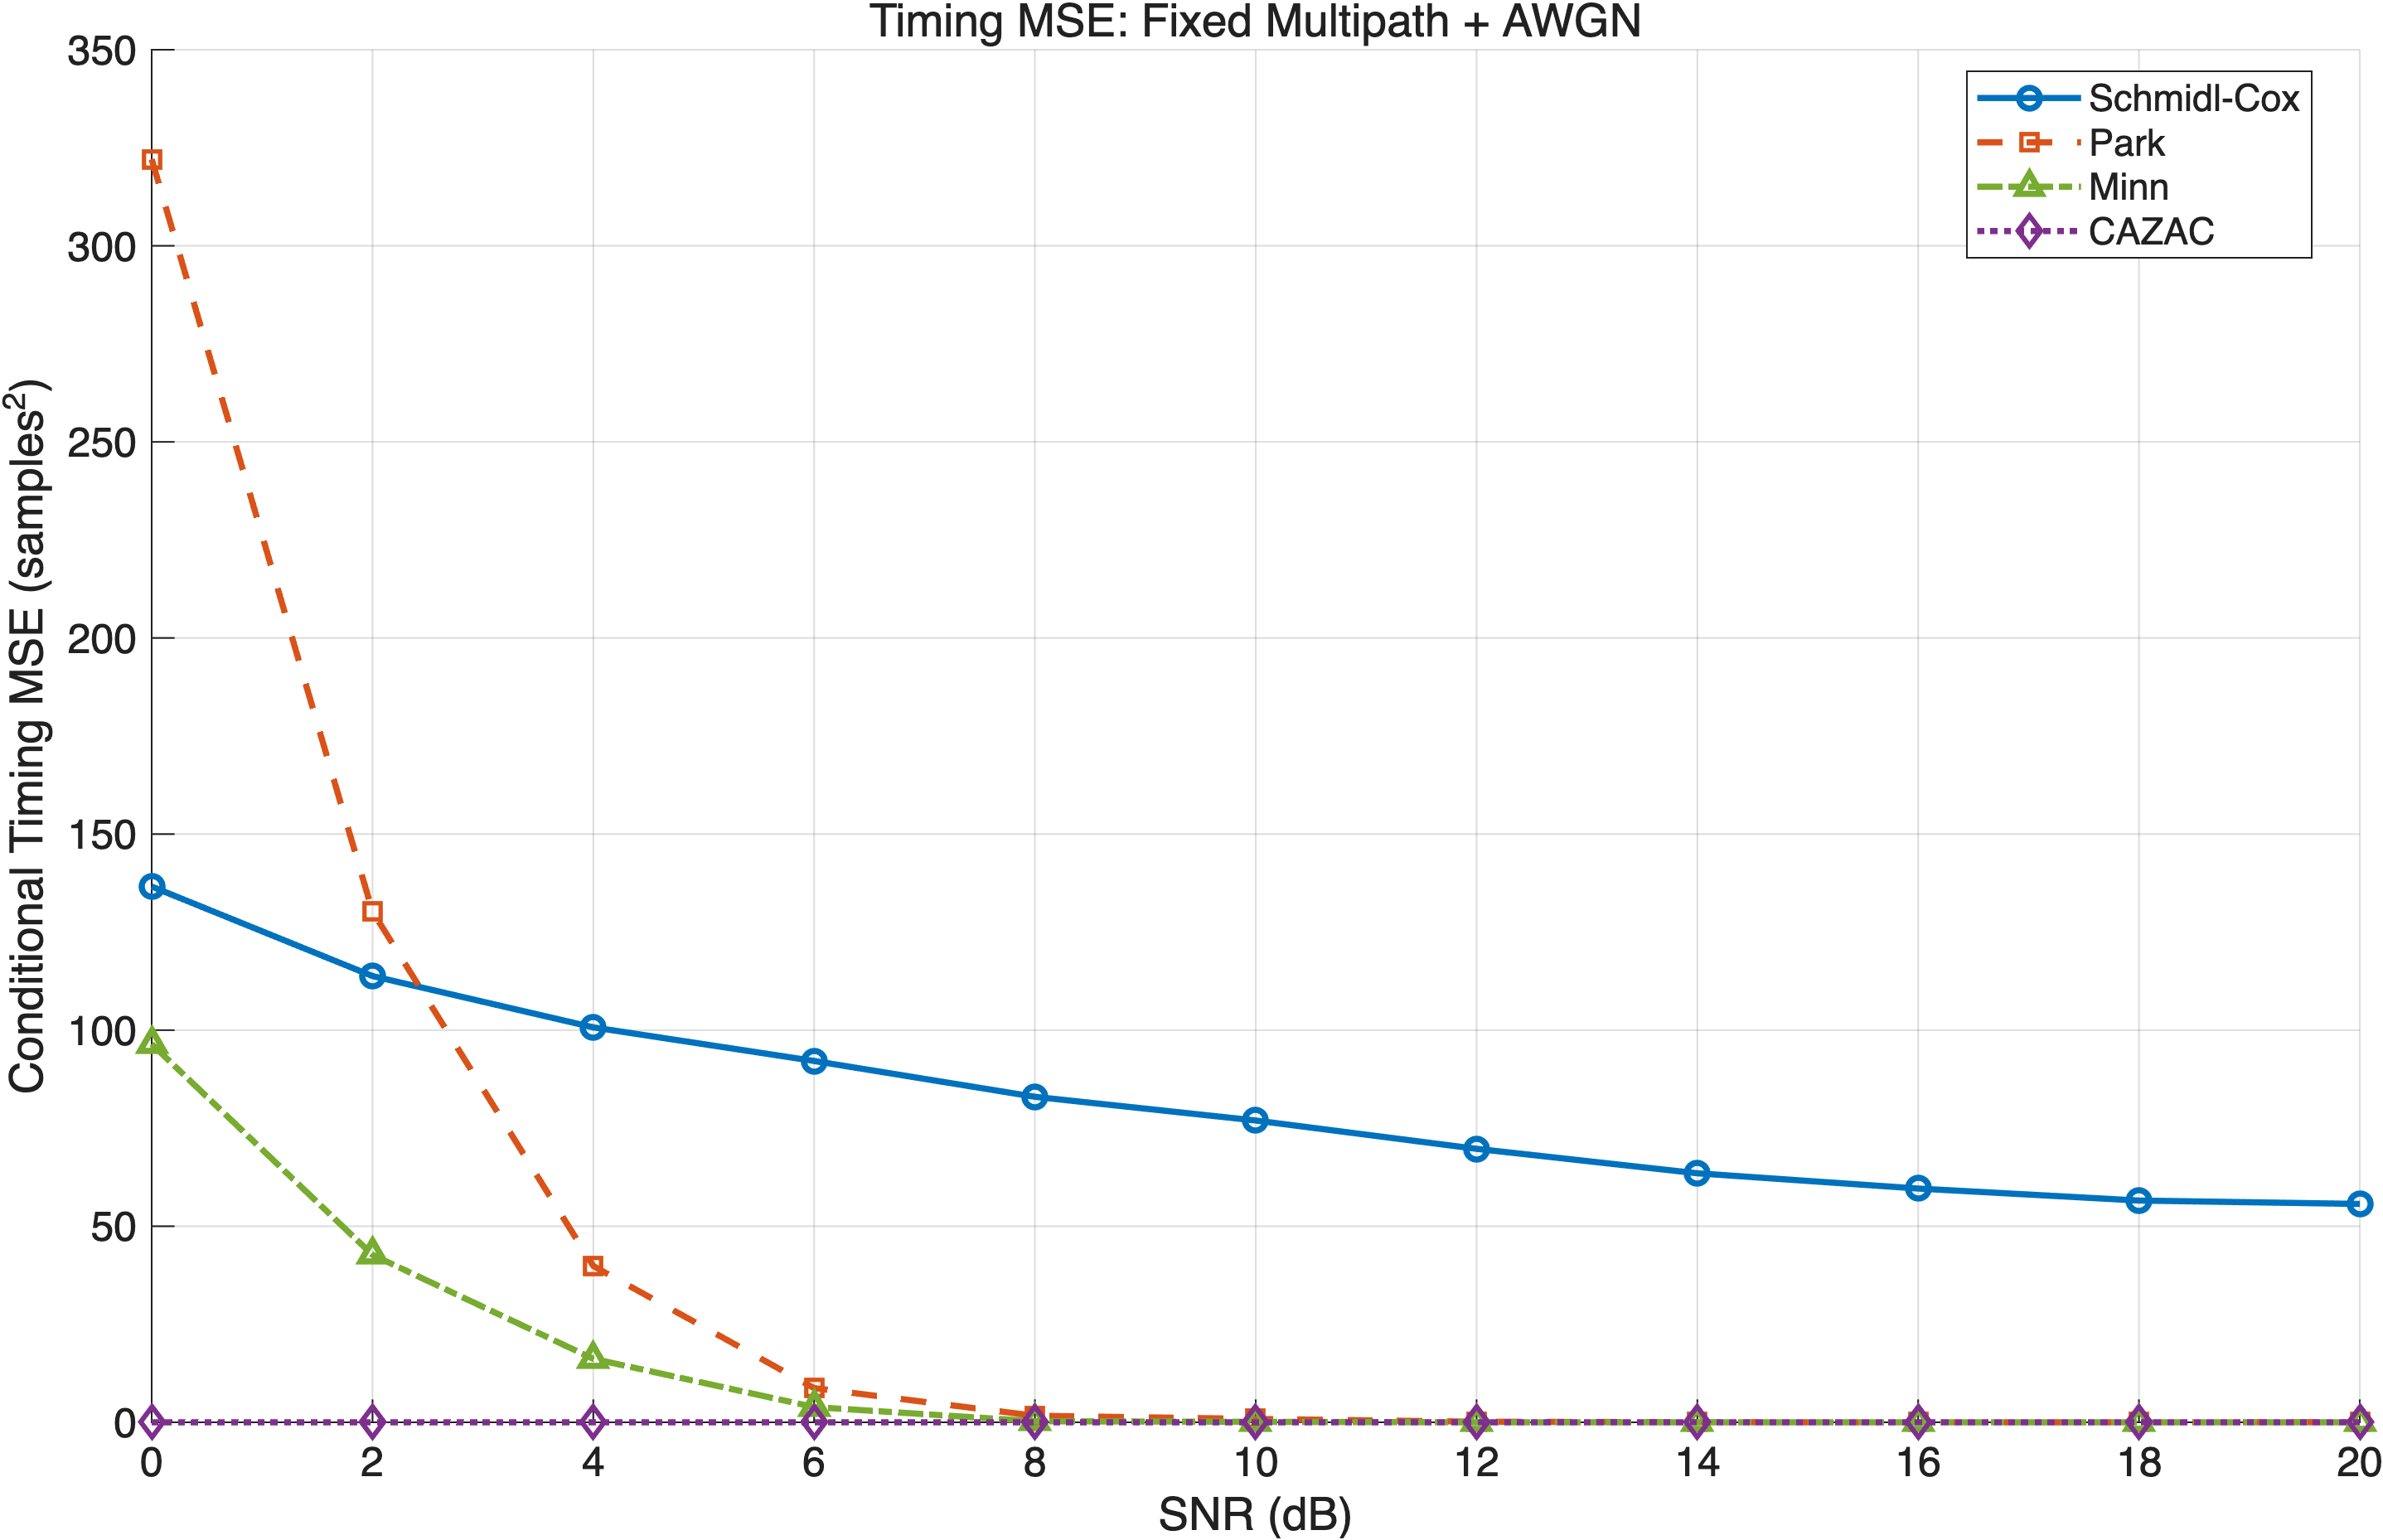
\includegraphics[width=0.84\linewidth,height=0.36\textheight,keepaspectratio]{figures/ch4/exp07_multipath_mse.png}\par\smallskip
{\small (b) Fixed multipath with AWGN}
\caption{EXP07: empirical timing MSE over the full SNR grid.}
\label{fig:ch4_mse}
\end{figure}

\begin{figure}[p]
\centering
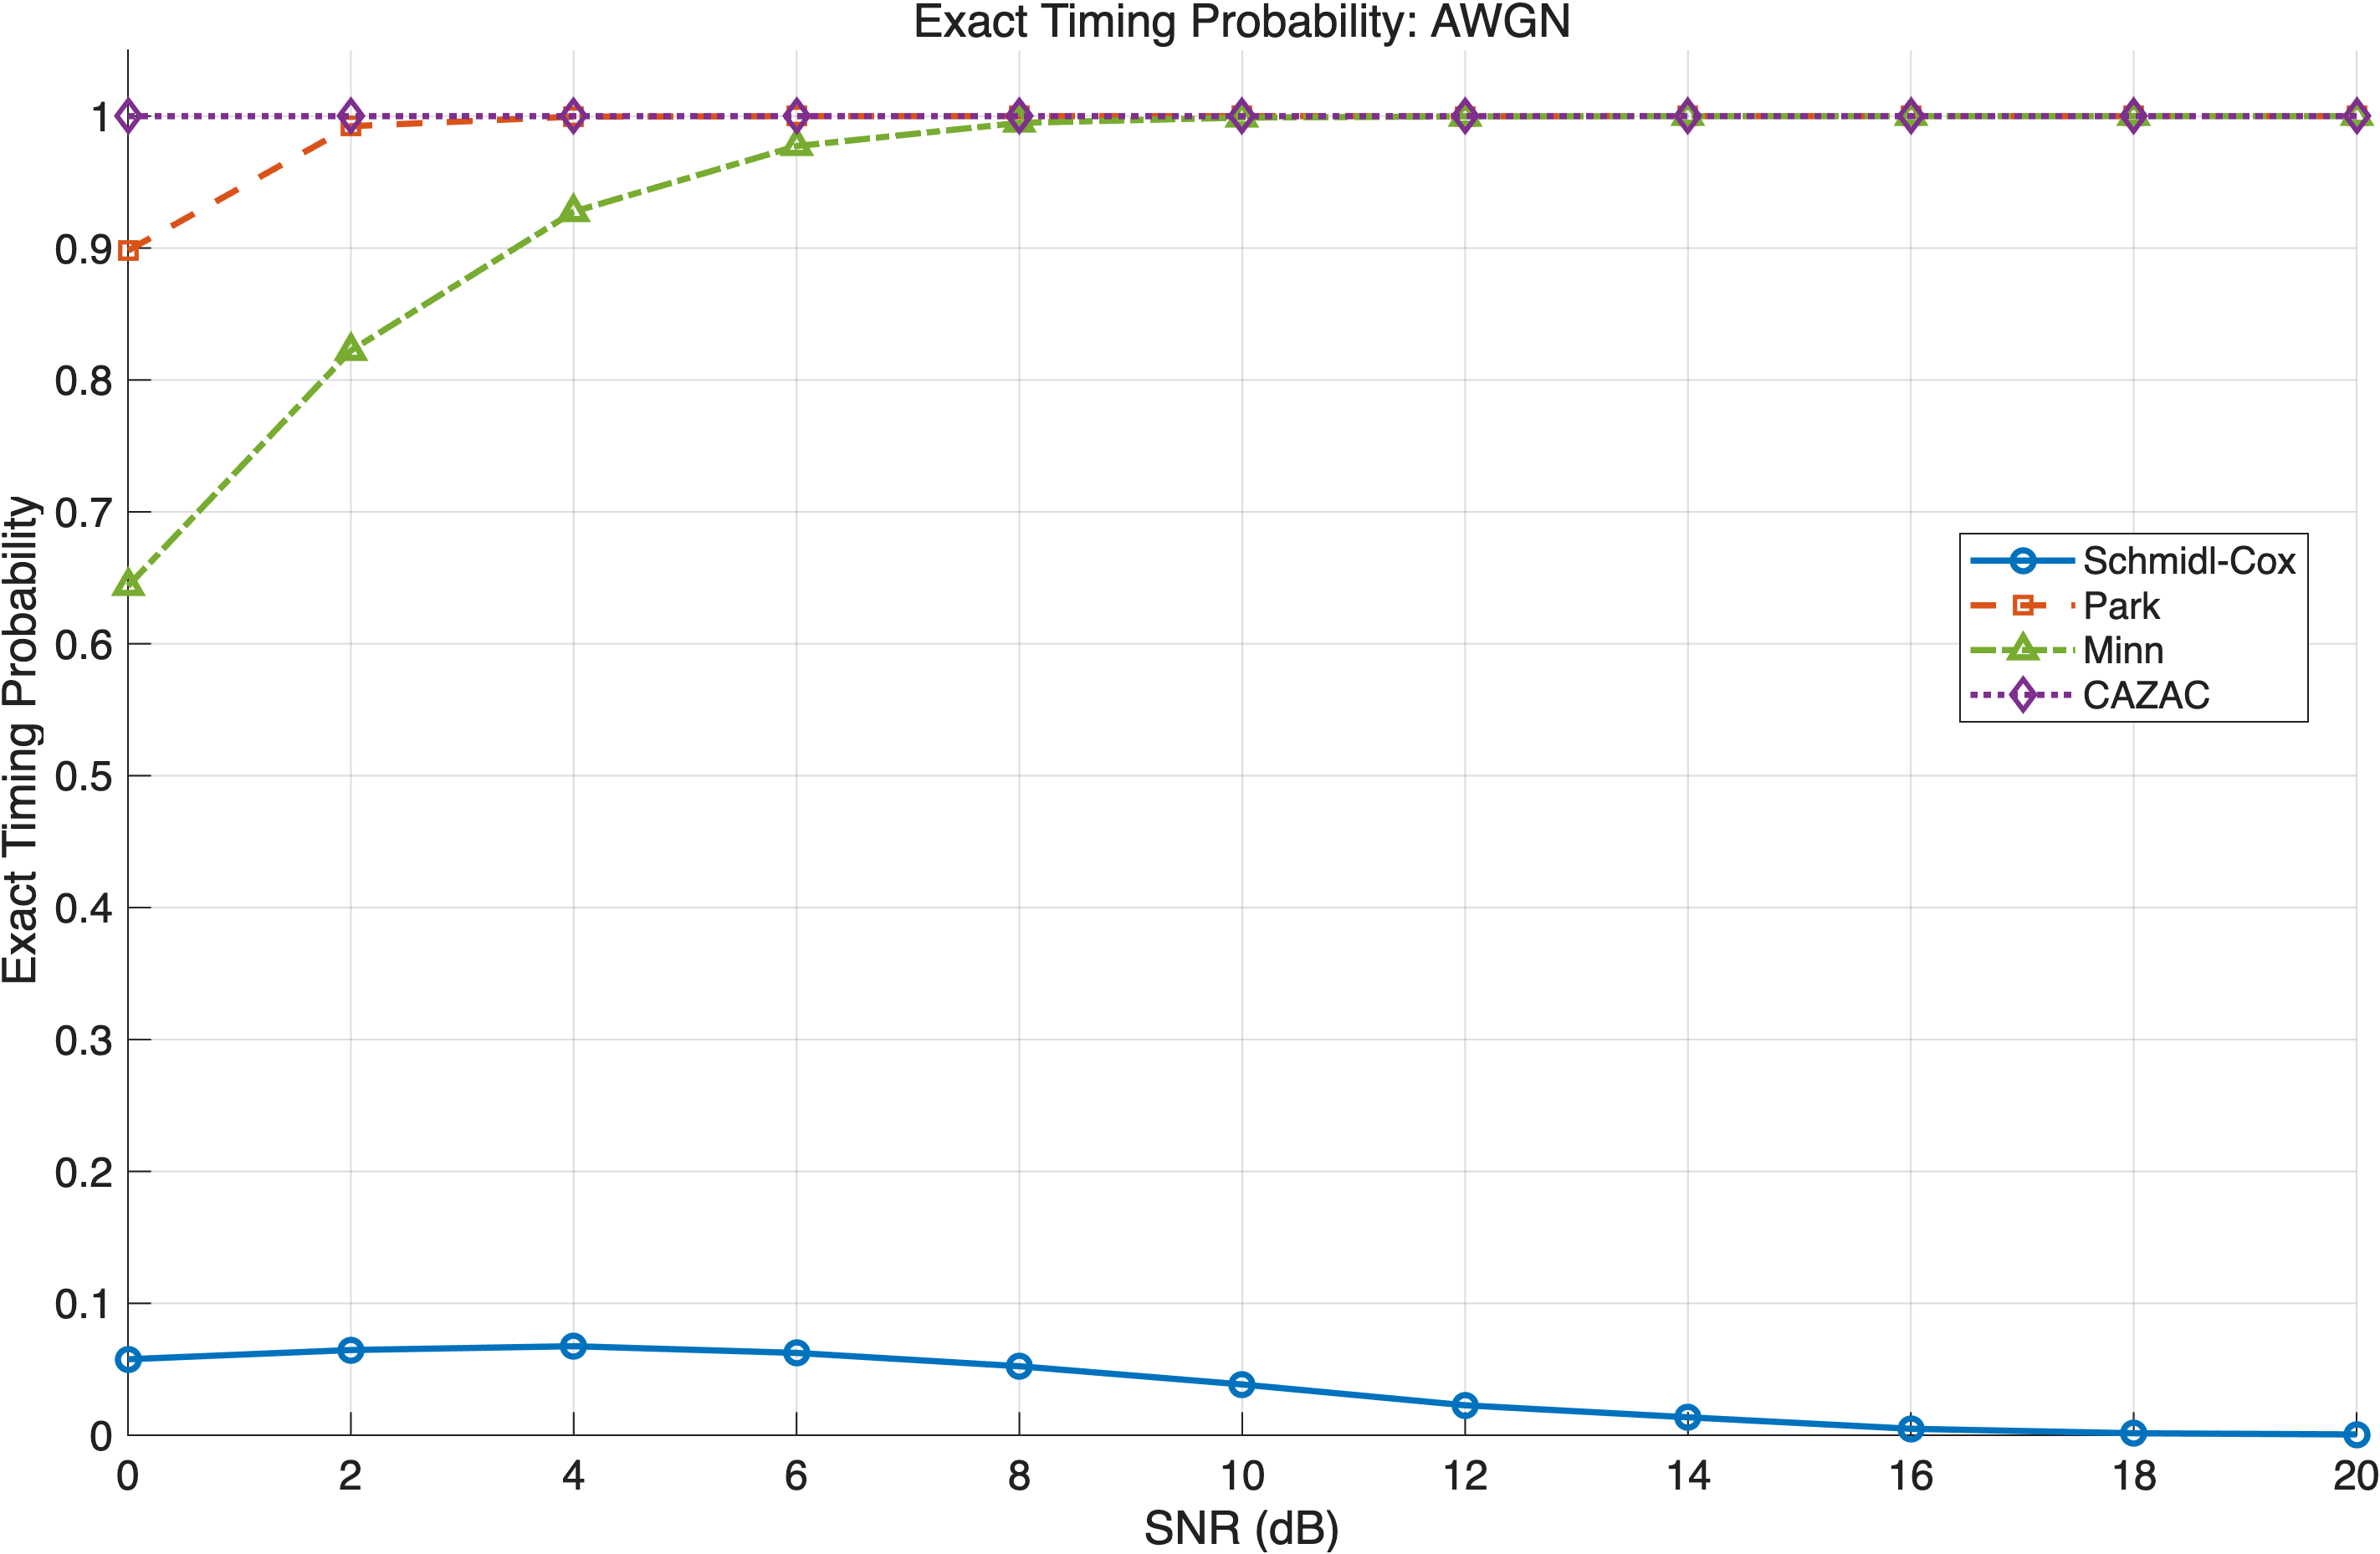
\includegraphics[width=0.84\linewidth,height=0.36\textheight,keepaspectratio]{figures/ch4/exp07_awgn_exact.png}\par\smallskip
{\small (a) AWGN}\par\medskip
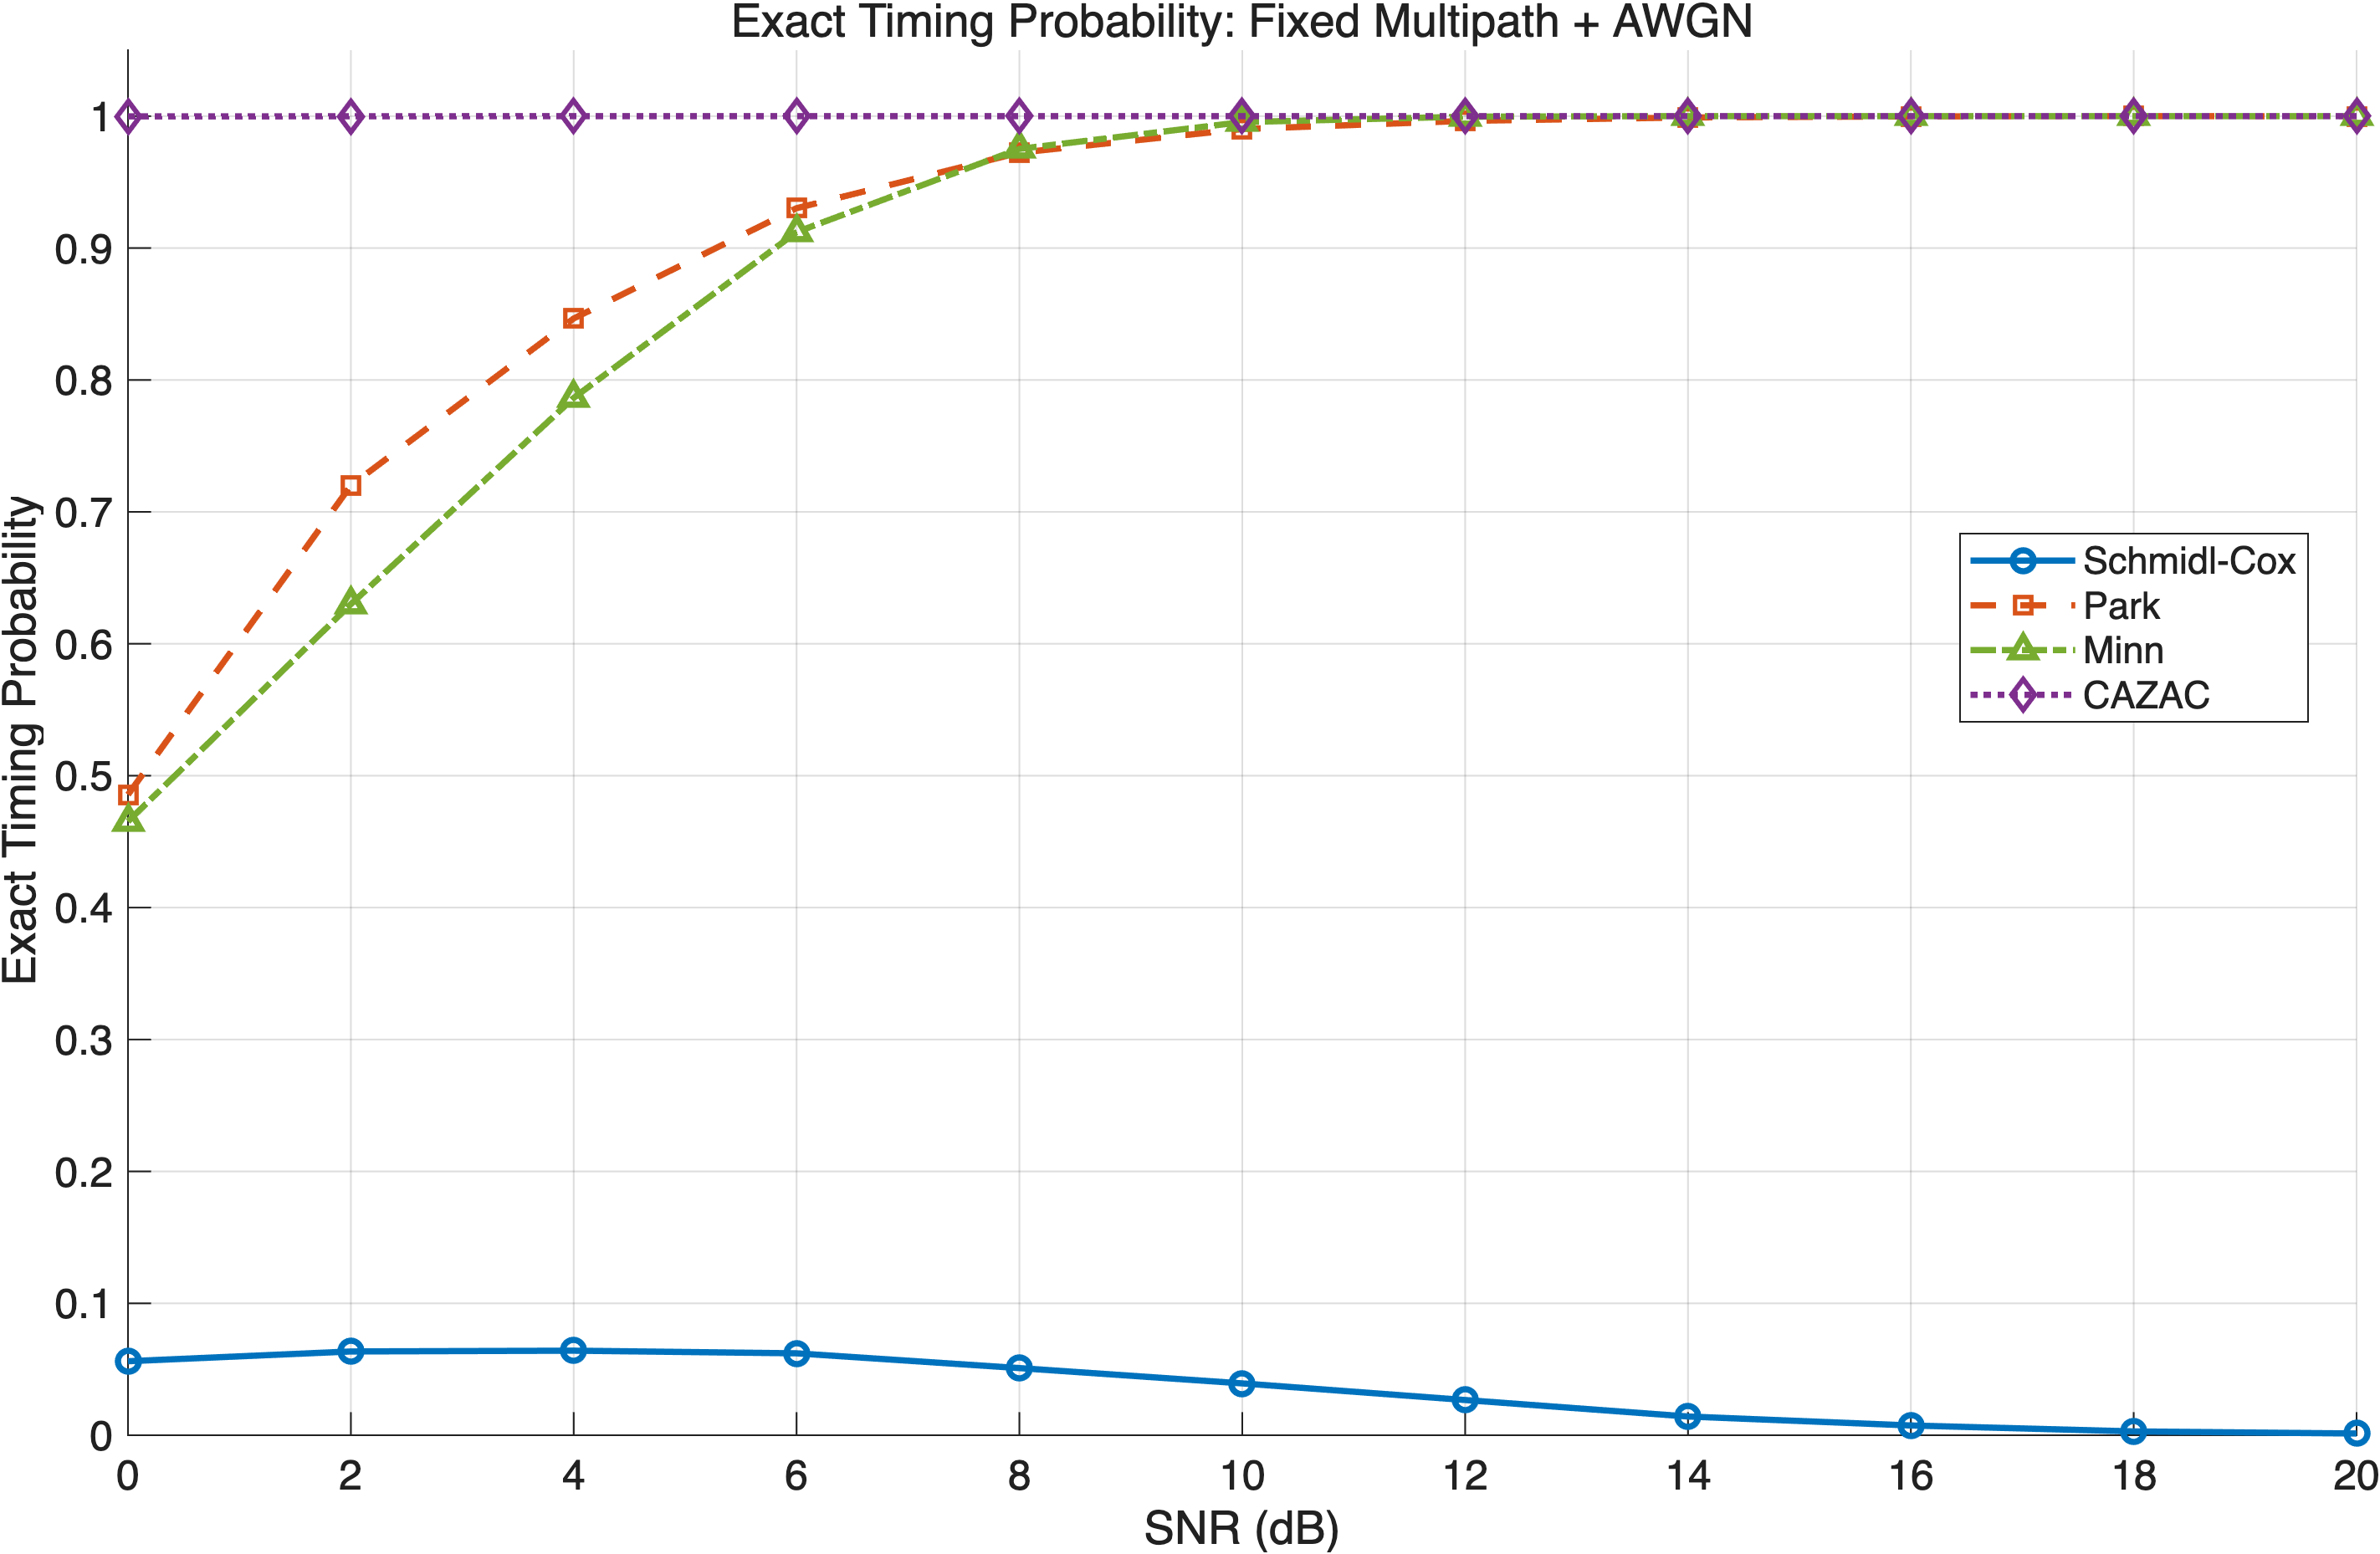
\includegraphics[width=0.84\linewidth,height=0.36\textheight,keepaspectratio]{figures/ch4/exp07_multipath_exact.png}\par\smallskip
{\small (b) Fixed multipath with AWGN}
\caption{EXP07: empirical exact-timing probability over the full SNR grid.}
\label{fig:ch4_exact}
\end{figure}

\begin{figure}[p]
\centering
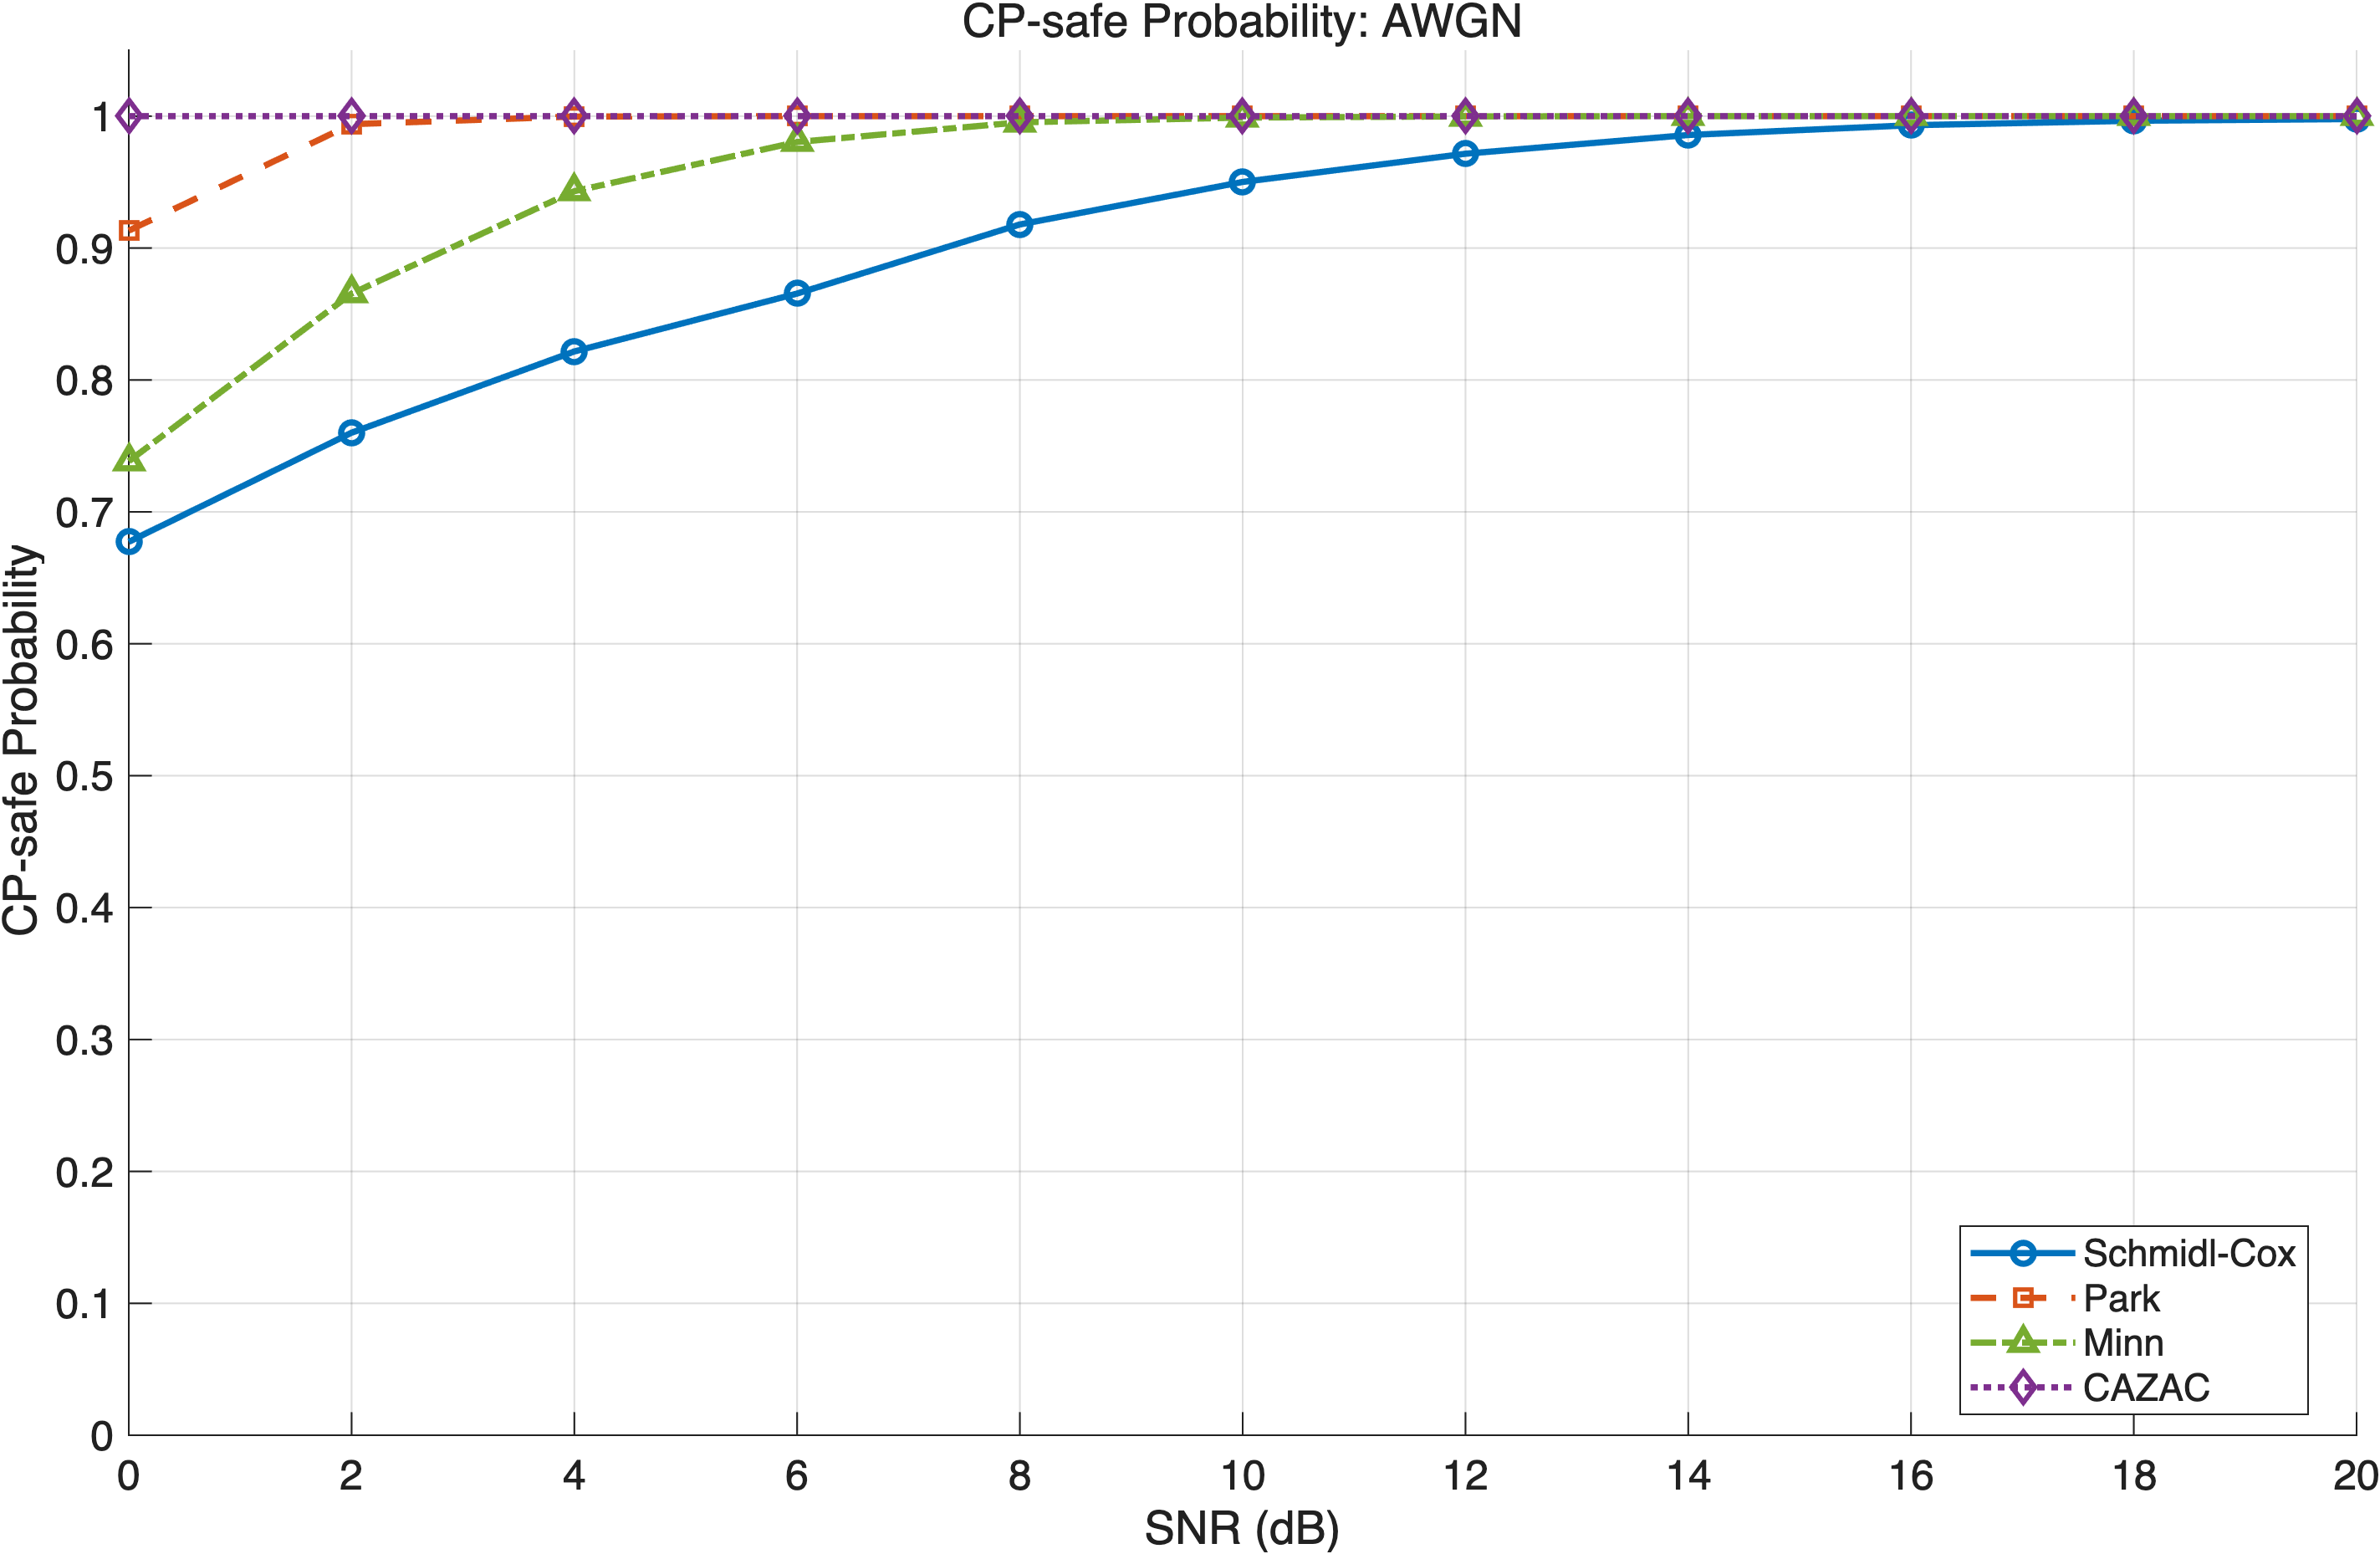
\includegraphics[width=0.84\linewidth,height=0.36\textheight,keepaspectratio]{figures/ch4/exp07_awgn_cpsafe.png}\par\smallskip
{\small (a) AWGN}\par\medskip
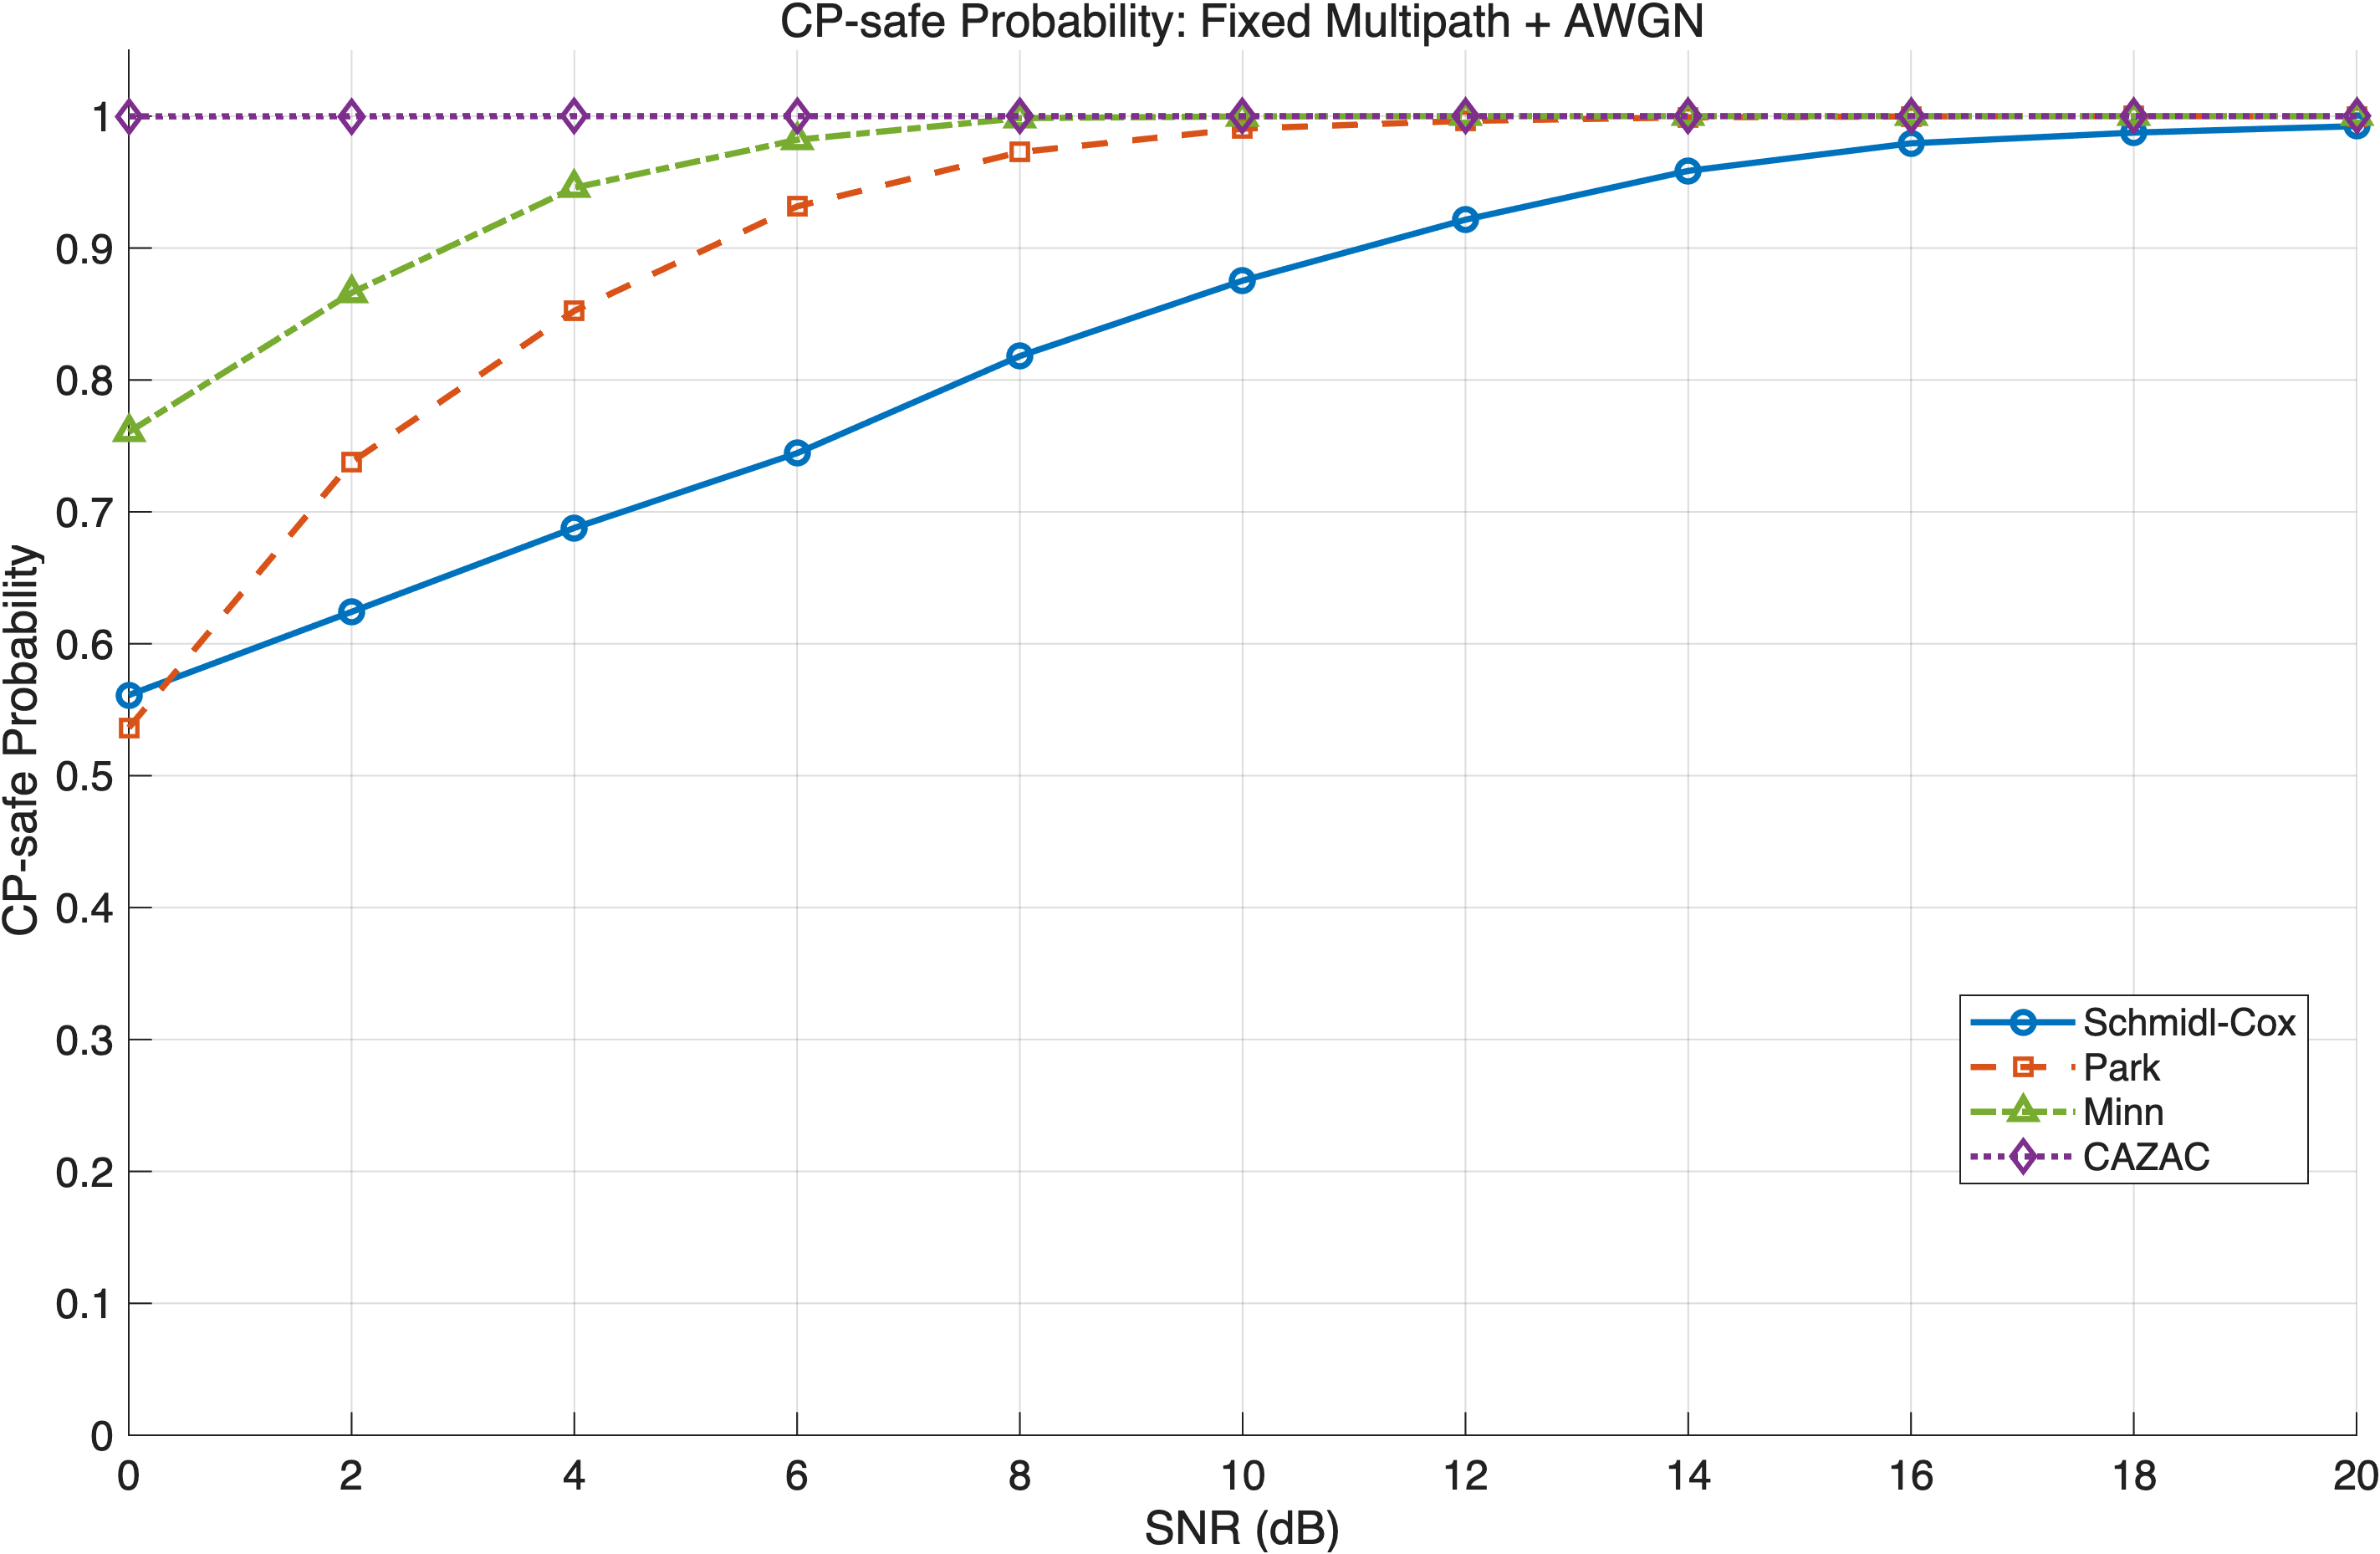
\includegraphics[width=0.84\linewidth,height=0.36\textheight,keepaspectratio]{figures/ch4/exp07_multipath_cpsafe.png}\par\smallskip
{\small (b) Fixed multipath with AWGN}
\caption{EXP07: empirical CP-safe probability over the full SNR grid. The safe intervals are $[-16,0]$ and $[-14,0]$ for (a) and (b), respectively.}
\label{fig:ch4_cpsafe}
\end{figure}

\subsection{Performance in AWGN}
At 0 dB, CAZAC has zero observed timing errors, Park achieves an exact probability of 0.8981, Minn 0.6438 and S\&C 0.0576. The corresponding MSE values for Park, Minn and S\&C are 100.1021, 116.1906 and 135.9962. As SNR increases, Park and Minn reduce their MSE rapidly; at 10 dB, Park has zero observed errors while Minn has MSE 0.9218 and exact probability 0.9989. At 20 dB, all three peak-based methods have zero observed errors.

The S\&C result differs qualitatively. Its MSE decreases from 135.9962 to 59.4513 between 0 and 20 dB, while CP-safe probability increases from 0.6773 to 0.9978. Yet the exact probability decreases to 0.0006 at 20 dB. A more stable metric leads to a more consistently early midpoint, not a more accurate estimate of the right-hand plateau boundary. Thus the improvement in safe-window placement is not equivalent to exact boundary acquisition.

\subsection{Performance in fixed multipath}
The fixed three-tap channel changes the estimator behavior most visibly at low SNR. At 0 dB, Park's exact probability falls from 0.8981 in AWGN to 0.4856 and its MSE rises to 322.0781. Minn has slightly lower exact probability (0.4653) but substantially lower MSE (96.4519) and higher CP-safe probability (0.7605) than Park (0.5363). Its errors are more often small or early enough to remain safe. The two criteria therefore produce different rankings. Minn's CP-safe probability at this point is also higher than its own AWGN value, despite the narrower acceptance interval; this is an empirical feature of this channel and error distribution, not a general benefit of multipath.

At 10 dB, Minn records exact and CP-safe probabilities of 0.9955 and 0.9998, with MSE 0.1140. Park records 0.9902 and 0.9905, with MSE 0.8639. S\&C reaches CP-safe probability 0.8753 but remains biased early. At 20 dB, Minn and CAZAC are exact in all 10,000 trials; Park has one nonzero error. S\&C reaches 0.9924 CP-safe probability but only 0.0013 exact probability. The S\&C MSE at 20 dB is somewhat smaller than in AWGN, which should not be interpreted as greater overall robustness: the safe interval has narrowed and the CP-safe probability is lower.

CAZAC's only errors in the unified experiment occur in fixed multipath at 0 and 2 dB: two and one estimates, respectively, are late by one sample. Across all 220,000 CAZAC estimates there are three nonzero errors. This high empirical accuracy is conditional on the selected deterministic channel, known template and bounded search range, not a universal performance guarantee.

\section[Error Distributions and Bias]{Timing-Error Distributions and Bias--Variance Analysis}
\label{sec:ch4_distribution}
The summary probabilities and MSE are complemented by the empirical distributions of the stored trial-level errors. Figures~\ref{fig:ch4_sc_hist}--\ref{fig:ch4_minn_hist} show three selected conditions, with bars representing percentages of all 10,000 trials and shaded regions indicating the integer CP-safe errors. These plots are derived from the EXP07 MAT arrays, rather than from the earlier individual-estimator experiments.

\begin{figure}[!htbp]
\centering
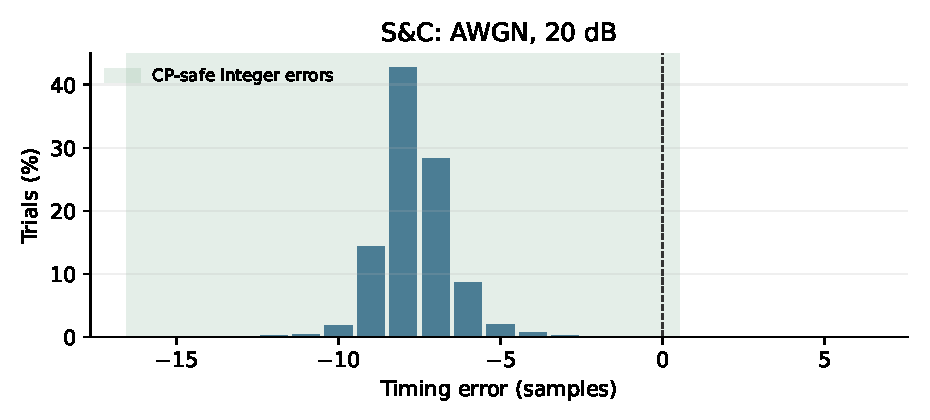
\includegraphics[width=1\linewidth]{figures/ch4/sc_awgn20_errors.pdf}
\caption{EXP07: S\&C timing-error distribution at 20 dB AWGN.}
\label{fig:ch4_sc_hist}
\end{figure}

\begin{figure}[!htbp]
\centering
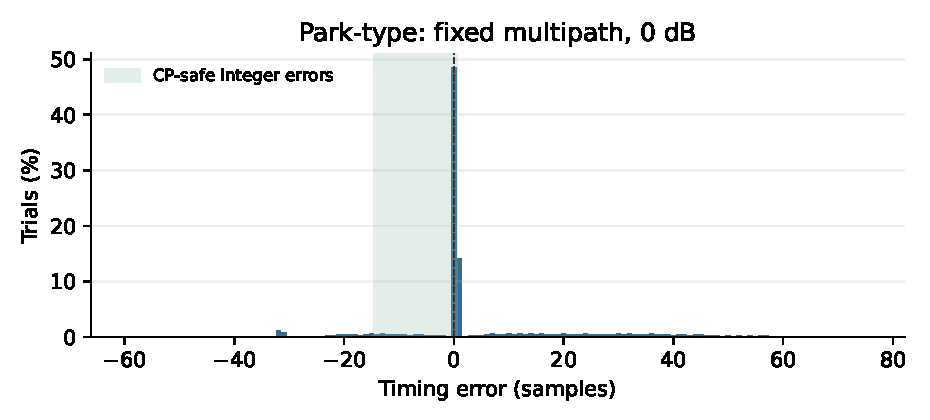
\includegraphics[width=1\linewidth]{figures/ch4/park_mp0_errors.pdf}
\caption{EXP07: Park-type timing-error distribution at 0 dB in fixed multipath.}
\label{fig:ch4_park_hist}
\end{figure}

\begin{figure}[!htbp]
\centering
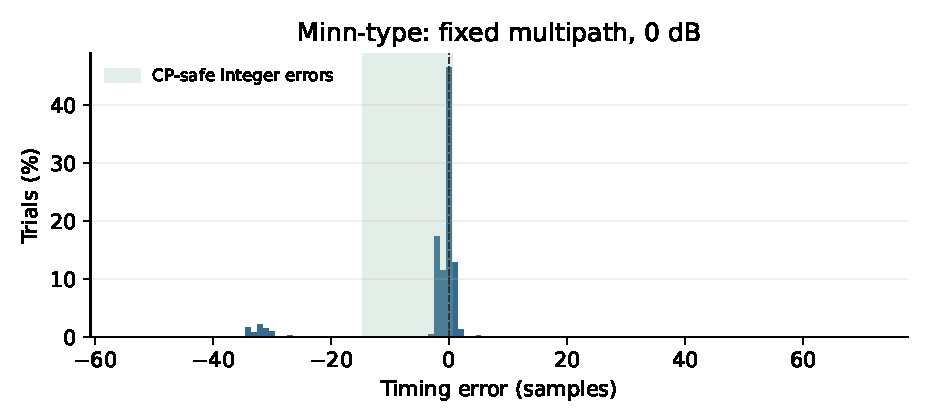
\includegraphics[width=1\linewidth]{figures/ch4/minn_mp0_errors.pdf}
\caption{EXP07: Minn-type timing-error distribution at 0 dB in fixed multipath.}
\label{fig:ch4_minn_hist}
\end{figure}

For S\&C at 20 dB AWGN, errors of $-8$ and $-7$ account for 4,278 and 2,824 trials, respectively. Only six trials give exact timing; 22 estimates are positive. The distribution is concentrated around an early offset rather than around zero. In contrast, Park at 0 dB multipath produces 4,856 exact estimates and 1,420 estimates at $+1$, with 2,508 errors of absolute magnitude at least 16 samples. Minn has 4,653 exact estimates and 1,737 at $-2$; 225 trials have error $-32$ and 905 errors have absolute magnitude at least 16. The latter secondary mode is consistent with the competing metric peak observed in the representative curves, although the stored errors alone do not prove the origin of every individual erroneous decision.

\begin{table}[htbp]
\centering
\caption{EXP07 bias--variance decomposition for selected conditions. Variance uses the denominator 10,000.}
\label{tab:ch4_biasvar}
\small
\begin{tabular}{llrrrr}
\hline
Channel, dB & Method & $\bar e$ & $\bar e^2$ & $v_K$ & MSE\\
\hline
AWGN, 20 & S\&C & $-7.6081$ & 57.8832 & 1.5681 & 59.4513\\
MP, 20 & S\&C & $-7.2907$ & 53.1543 & 2.5276 & 55.6819\\
MP, 0 & Park & 4.9677 & 24.6780 & 297.4001 & 322.0781\\
MP, 0 & Minn & $-2.9189$ & 8.5200 & 87.9319 & 96.4519\\
\hline
\end{tabular}
\end{table}

Table~\ref{tab:ch4_biasvar} decomposes MSE using the empirical identity from Section 2.9. In AWGN at 20 dB, approximately 97.36\% of S\&C MSE is squared bias; in multipath at 20 dB the proportion is approximately 95.46\%. The high-SNR limitation is systematic rather than predominantly random. By contrast, at 0 dB multipath, the variance term accounts for about 92.34\% of Park MSE and 91.17\% of Minn MSE. Large errors strongly influence the squared-error criterion even when many estimates are exact.

Rare errors also explain some apparent irregularities at high SNR. For example, Minn at 10 dB AWGN has nine errors of $-32$ and two of $+1$ among 10,000 trials. The nine large errors contribute $9(32)^2/10000=0.9216$ of its MSE of 0.9218. Park at 20 dB multipath has one error of $+19$, producing the entire MSE of 0.0361 despite 9,999 exact estimates. Its MSE was zero at 18 dB; the increase at the next tested SNR should not be interpreted as evidence of systematic deterioration. The empirical curve is sensitive to rare events and finite simulation size.

\section[Statistical Interpretation]{Statistical Interpretation and Robustness}
\label{sec:ch4_statistical}
With 10,000 trials in a condition, probability estimates have a resolution of 0.0001. Under independent trials at a fixed condition, the binomial standard error is $\sqrt{p(1-p)/10000}$, at most 0.005. For example, the plug-in standard errors of Park and Minn exact probability at 0 dB multipath are both close to 0.005. Since the methods share trial scenarios, comparisons between them should not be treated as tests of two independent proportions. This chapter uses descriptive comparisons rather than claiming formal statistical significance from separate marginal standard errors.

When no nonexact estimates are observed in 10,000 trials, a one-sided 95\% binomial upper bound on the nonexact probability is $1-0.05^{1/10000}\approx 0.000300$, assuming independent trials with a common probability for that condition. This illustrates the finite-sample uncertainty even when the reported exact probability equals one. The bound is per condition and is not a simultaneous guarantee over the full SNR grid. All reported zero MSE and zero failure values are empirical observations.

The primary comparison identifies three distinct patterns: plateau-induced bias for S\&C, noise- and channel-sensitive peak selection for Park and Minn, and very reliable known-template matching for CAZAC in the tested model. Identical transmitted energy and a common candidate support make the comparison more controlled, but do not equalize the information used by each estimator. The results characterize the four selected implementations under the stated simulation conditions. They do not establish that a specific algorithm is universally optimal or that its performance is unchanged under other channel profiles, frequency offsets or fractional delays.

\section{Chapter Summary}
EXP01 and EXP02 verify the OFDM processing model and distinguish phase rotation from loss of the circular-convolution structure. EXP07 shows that exact timing, CP-safe timing and MSE describe distinct properties. A method may place most windows within the safe interval while retaining systematic bias, or achieve a high exact probability while suffering large MSE due to rare errors. Chapter 5 uses EXP08 to examine their consequences for data detection.
